\chapter{HASIL DAN PEMBAHASAN}

\section{Perancangan \textit{(Exploration Phase)}}

\subsection{\textit{Requirements}}

Pada fase ini, seluruh kebutuhan pengguna akan dikumpulkan dalam bentuk \textit{user story}. Seluruh \textit{user story} akan diubah menjadi \textit{task} yang dapat dikerjakan pada jangka waktu tertentu yang disebut dengan iterasi. Pada metode \textit{Extreme Programming}, iterasi dapat berlangsung selama 1 hingga 2 pekan. Dalam penelitian ini, 1 iterasi akan ditetapkan berlangsung selama 1 pekan. \textit{User story} pada penelitian ini dapat dilihat pada tabel dibawah.

\begin{longtable}[!h]
    {
            p{0.15\textwidth}
            p{0.15\textwidth}
            p{0.35\textwidth}
            p{0.35\textwidth}
    }
    \caption{Daftar \textit{user story} Sistem Monitoring}
    \label{tab:user-story-fix} \\

    \hline
        \bfseries \textit{Code} &
        \bfseries \textit{Persona} &
        \bfseries \textit{I want to} &
        \bfseries \textit{So that can} \\ [0.5ex]
    \hline

    \endfirsthead

    \hline
        \bfseries \textit{Code} &
        \bfseries \textit{Persona} &
        \bfseries \textit{I want to} &
        \bfseries \textit{So that can} \\ [0.5ex]
    \hline
    \endhead % all the lines above this will be repeated on every page
    \hline

    \csvreader[
        late after line=\\,
        before reading={\catcode`\#=12},after reading={\catcode`\#=6}
    ]{tables/hasil/user-story.csv}{1=\K, 2=\P, 3=\I, 4=\S}{\K & \P & \I & \S} \\

    \bottomrule
\end{longtable}

\subsection{Architecture Modelling}

Dalam buku \textit{Fundamental of Software Architecture} oleh \textcite{book:richard}, arsitektur didefinisikan sebagai sebuah rangkaian dari keputusan yang akan menentukan struktur dan perilaku sistem. Pada metode XP, model arsitektur dibuat untuk mempertimbangkan berbagai solusi alternatif. Model arsitektur pada Sistem Monitoring dapat dilihat pada Gambar \ref{fig:archi-model-sm} .

\begin{figure}[!h]
    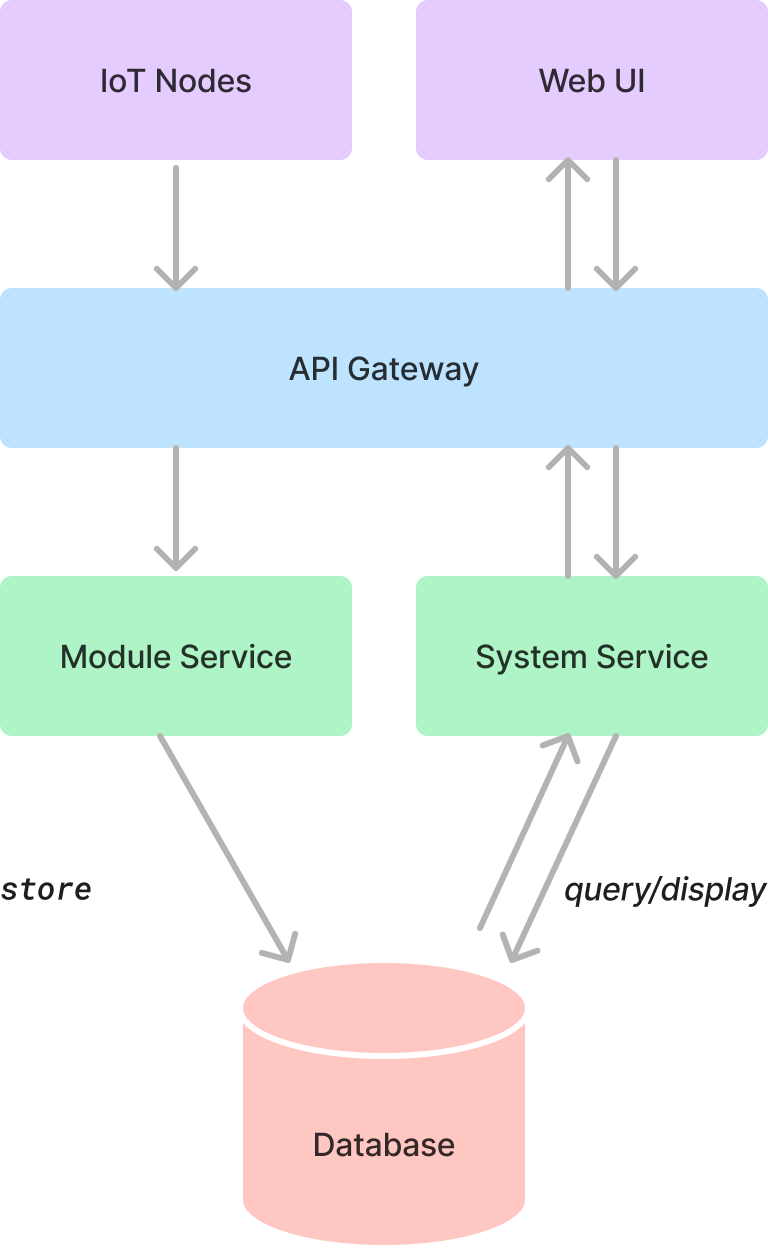
\includegraphics[width=.4\linewidth, center]{images/hasil/archi-model.png}
    \caption{Metafor Model Arsitektur Sistem Monitoring}
    \label{fig:archi-model-sm}
\end{figure}

Gambar di atas merupakan model arsitektur dengan style \textit{Service-based Architecture} dengan pertimbangan bahwa sistem tidak hanya menyediakan \textit{(API Gateway)} untuk web dasbor saja, melainkan juga untuk perangkat IoT yang akan dipasang di kapal, disebut juga dengan \textit{IoT Nodes}. \textit{IoT Nodes} dapat mengirimkan data dengan mengirimkan \textit{HTTP Request} ke server melalui \textit{(API Gateway)} yang telah diatur pada \textit{Module Service} untuk meneruskan data ke \textit{Database}. Data yang telah tersimpan dapat diakses melalui \textit{Web UI} yang terhubung dengan \textit{System Service} melalui \textit{(API Gateway)}. Selain mengakses data, sistem juga memungkinkan pengguna untuk dapat melakukan filter data dengan memberi input tanggal yang ditunjukkan oleh dua garis penghubung pada setiap obyek yang menghubungkan \textit{Web UI} dengan \textit{Database}.

\subsection{Tools dan Teknologi}

Selama pengembangan sistem, digunakan beberapa \textit{tools} yang akan membantu proses tersebut serta pemilihan teknologi \textit{(techstack)} untuk Sistem Monitoring yang sebelumnya telah dibahas pada Bab 2 dan Bab 3. Untuk tools yang digunakan dalam penelitian ini meliputi VSCode sebagai IDE, phpmyadmin untuk melakukan manajemen basis data, Figma untuk mendesain arsitektur, skema basis data, dan prototype, serta Apidog untuk pengujian API.

\section{Perencanaan \textit{(Planning)}}

\subsection{Rencana Awal \textit{(Initial Planning)}}

Pada tahap ini, seluruh \textit{User Story} akan menjadi kumpulan \textit{task} yang akan disortir berdasarkan tingkat prioritas yang dinilai dari 1 hingga 5 dan estimasi waktu pengerjaannya dalam satuan hari. Seluruh rencana iterasi dapat dilihat pada Tabel \ref{tab:iteration-1} hingga Tabel \ref{tab:iteration-5} dibawah.

Iterasi pertama difokuskan untuk mengelola data kecepatan mesin dan menampilkannya dalam bentuk grafik.

\begin{longtable}[!h]
    {
            p{0.2\textwidth}
            p{0.4\textwidth}
            >{\centering\arraybackslash}p{0.15\textwidth}
            >{\centering\arraybackslash}p{0.15\textwidth}
    }
    \caption{Rencana Iterasi 1}
    \label{tab:iteration-1} \\

    \hline
        \bfseries \textit{Kode User Story} &
        \bfseries \textit{Deskripsi Task} &
        \bfseries \textit{Prioritas} &
        \bfseries \textit{Estimasi Waktu} \\ [0.5ex]
    \hline

    \endfirsthead

    \hline
        \bfseries \textit{Kode User Story} &
        \bfseries \textit{Deskripsi} &
        \bfseries \textit{Prioritas} &
        \bfseries \textit{Estimasi Waktu} \\ [0.5ex]
    \hline
    \endhead % all the lines above this will be repeated on every page
    \hline

    \csvreader[
        late after line=\\,
        before reading={\catcode`\#=12},after reading={\catcode`\#=6}
    ]{tables/hasil/iterations/1/task.csv}
    {1=\K, 2=\D, 3=\P, 4=\T}{\K & \D & \P & \T} \\

    \bottomrule
\end{longtable}

Pada iterasi kedua, dilanjutkan pengembangan Halaman Fuel Consumption, Running Hour, dan Data Log.

\begin{longtable}[!h]
    {
            p{0.15\textwidth}
            p{0.4\textwidth}
            >{\centering\arraybackslash}p{0.15\textwidth}
            >{\centering\arraybackslash}p{0.15\textwidth}
    }
    \caption{Rencana Iterasi 2}
    \label{tab:iteration-2} \\

    \hline
        \bfseries Kode User Story &
        \bfseries Deskripsi Task &
        \bfseries Prioritas &
        \bfseries Estimasi Waktu \\ [0.5ex]
    \hline

    \endfirsthead

    \hline
        \bfseries Kode User Story &
        \bfseries Deskripsi &
        \bfseries Prioritas &
        \bfseries Estimasi Waktu \\ [0.5ex]
    \hline
    \endhead % all the lines above this will be repeated on every page
    \hline

    \csvreader[
        late after line=\\,
        before reading={\catcode`\#=12},after reading={\catcode`\#=6}
    ]{tables/hasil/iterations/2/task.csv}
    {1=\c, 2=\d, 3=\p, 4=\t}{\c & \d & \p & \t} \\

    \bottomrule
\end{longtable}

Selanjutnya, pada iterasi ketiga dilakukan pengembangan sistem admin yang memungkinkan pengguna melakukan manajemen data seperti data pengguna, data kapal, dan data batas kecepatan pada setiap kategori operasional FCRV.

\begin{longtable}[!h]
    {
            p{0.15\textwidth}
            p{0.4\textwidth}
            >{\centering\arraybackslash}p{0.15\textwidth}
            >{\centering\arraybackslash}p{0.15\textwidth}
    }
    \caption{Rencana Iterasi 3}
    \label{tab:iteration-3} \\

    \hline
        \bfseries Kode User Story &
        \bfseries Deskripsi Task &
        \bfseries Prioritas &
        \bfseries Estimasi Waktu \\ [0.5ex]
    \hline

    \endfirsthead

    \hline
        \bfseries Kode User Story &
        \bfseries Deskripsi &
        \bfseries Prioritas &
        \bfseries Estimasi Waktu \\ [0.5ex]
    \hline
    \endhead % all the lines above this will be repeated on every page
    \hline

    \csvreader[
        late after line=\\,
        before reading={\catcode`\#=12},after reading={\catcode`\#=6}
    ]{tables/hasil/iterations/3/task.csv}
    {1=\c, 2=\d, 3=\p, 4=\t}{\c & \d & \p & \t} \\

    \bottomrule
\end{longtable}

Iterasi keempat berfokus pada pembuatan laporan harian kecepatan mesin dan konsumsi bahan bakar dalam format PDF.

\begin{longtable}[!h]
    {
            p{0.15\textwidth}
            p{0.4\textwidth}
            >{\centering\arraybackslash}p{0.15\textwidth}
            >{\centering\arraybackslash}p{0.15\textwidth}
    }
    \caption{Rencana Iterasi 4}
    \label{tab:iteration-4} \\

    \hline
        \bfseries Kode User Story &
        \bfseries Deskripsi Task &
        \bfseries Prioritas &
        \bfseries Estimasi Waktu \\ [0.5ex]
    \hline

    \endfirsthead

    \hline
        \bfseries Kode User Story &
        \bfseries Deskripsi &
        \bfseries Prioritas &
        \bfseries Estimasi Waktu \\ [0.5ex]
    \hline
    \endhead % all the lines above this will be repeated on every page
    \hline

    \csvreader[
        late after line=\\,
        before reading={\catcode`\#=12},after reading={\catcode`\#=6}
    ]{tables/hasil/iterations/4/task.csv}
    {1=\c, 2=\d, 3=\p, 4=\t}{\c & \d & \p & \t} \\

    \bottomrule
\end{longtable}

Terakhir, pada iterasi kelima dilakukan pengembangan sistem autentikasi dan juga ekspor data mentah kecepatan mesin dalam format CSV.

\begin{longtable}[!h]
    {
            p{0.2\textwidth}
            p{0.4\textwidth}
            >{\centering\arraybackslash}p{0.15\textwidth}
            >{\centering\arraybackslash}p{0.15\textwidth}
    }
    \caption{Rencana Iterasi 5}
    \label{tab:iteration-5} \\

    \hline
        \bfseries \textit{Kode User Story} &
        \bfseries \textit{Deskripsi Task} &
        \bfseries \textit{Prioritas} &
        \bfseries \textit{Estimasi Waktu} \\ [0.5ex]
    \hline

    \endfirsthead

    \hline
        \bfseries \textit{Kode User Story} &
        \bfseries \textit{Deskripsi} &
        \bfseries \textit{Prioritas} &
        \bfseries \textit{Estimasi Waktu} \\ [0.5ex]
    \hline
    \endhead % all the lines above this will be repeated on every page
    \hline

    \csvreader[
        late after line=\\,
        before reading={\catcode`\#=12},after reading={\catcode`\#=6}
    ]{tables/hasil/iterations/5/task.csv}
    {1=\K, 2=\D, 3=\P, 4=\T}{\K & \D & \P & \T} \\

    \bottomrule
\end{longtable}

\subsection{Perubahan \textit{(Changes)}}

Selama pengerjaan berlangsung, terdapat beberapa umpan balik dari mitra yang mengakibatkan penambahan pada task. Sehingga, ini juga berdampak pada rencana iterasi yang sebelumnya telah dibuat. Secara garis besar, task yang bertambah adalah sistem admin untuk melakukan manajemen data kapal, manajemen data pengguna, manajemen data FCRV. Hasil akhir, terdapat task dengan total sebanyak 13 item yang dikerjakan selama 5 iterasi.

\begin{longtable}[!h]
    {
            p{0.15\textwidth}
            p{0.4\textwidth}
            p{0.2\textwidth}
            p{0.2\textwidth}
    }
    \caption{Umpan Balik Selama Pengembangan}
    \label{tab:feedback} \\

    \hline
        \bfseries No &
        \bfseries Umpan Balik &
        \bfseries Iterasi &
        \bfseries Status \\ [0.5ex]
    \hline

    \endfirsthead

    \hline
        \bfseries No &
        \bfseries Umpan Balik &
        \bfseries Iterasi &
        \bfseries Status \\ [0.5ex]
    \hline
    \endhead % all the lines above this will be repeated on every page
    \hline

    \csvreader[
        late after line=\\,
        before reading={\catcode`\#=12},after reading={\catcode`\#=6}
    ]{tables/hasil/changes.csv}{1=\no, 2=\feedback, 3=\i, 4=\status}{\no & \feedback & \i & \status} \\

    \bottomrule
\end{longtable}

Setelah mendapat kebutuhan awal, terdapat permintaan tambahan untuk membangun sistem admin agar mitra dapat lebih leluasa untuk melakukan konfigurasi data. Sistem admin meliputi manajemen data pengguna, data kapal, dan data FCRV. Setelah direkap di user story dan dilakukan skala prioritas, pengembagan Sistem Admin akan dilakukan pada iterasi 3.
Pada iterasi kedua, terdapat permintaan untuk mencantumkan angka running hour pada halaman engine speed yang diposisikan dibawah angka kecepatan mesin. Sedangkan pada iterasi 5, terdapat permintaan untuk menambah 2 halaman, yakni Home dan OP41 Report. Halaman Home berisi seluruh kapal yang terdaftar dan Halaman OP41 Report berisi laporan konsumsi bahan bakar berdasarkan perhitungan dari kategori FCRV yang dapat dilihat pada Lampiran \ref{apdx:coding}.


\section{Implementasi \textit{(Iteration to Release)}}

\begin{figure}[!h]
    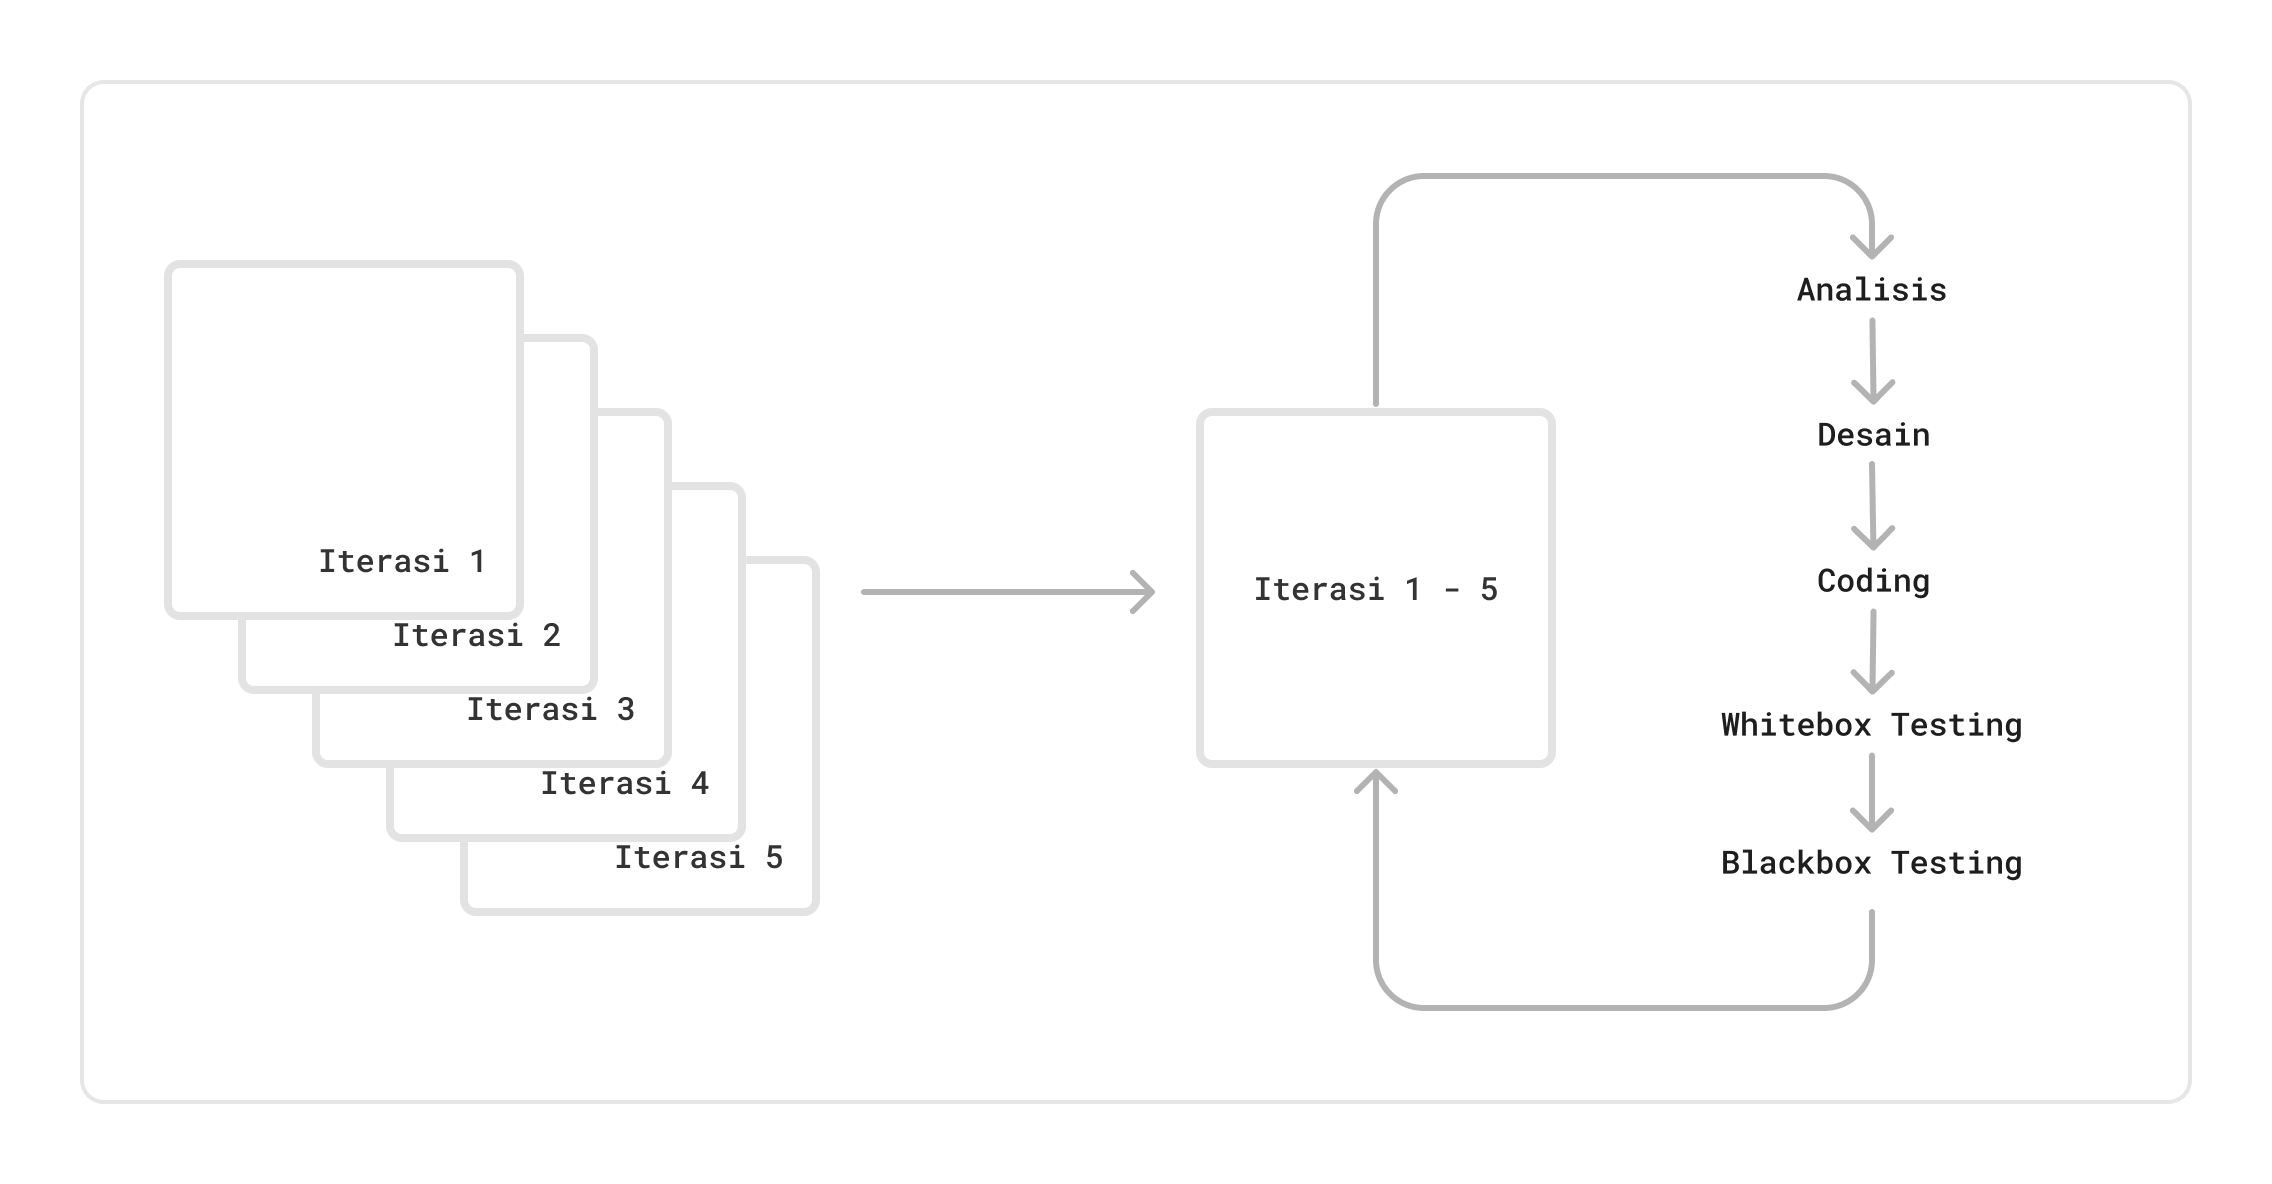
\includegraphics[width=1.05\linewidth, center]{images/hasil/overview.png}
    \caption{Garis Besar Pengerjaan Implementasi}
    \label{fig:imp-overview}
\end{figure}

Secara garis besar, implementasi dilakukan sebanyak 5 iterasi yang berlangsung selama 5 pekan seperti yang terlihat pada Gambar \ref{fig:imp-overview}. Dimulai dari tahap analisis yang akan menghasilkan kebutuhan sistem, dilanjutkan dengan perancangan \textit{wireframe} sebagai acuan pada pengembangan antarmuka di fase koding, yang akan melewati serangkaian proses pengujian yang disebut dengan \textit{Whitebox Testing} dan \textit{Blackbox Testing}. Pengujian \textit{whitebox} dilakukan untuk memastikan kesesuaian seluruh struktur dan logika pemrograman dengan melalui \textit{unit test}. Lalu, setelahnya dilakukan pengujian langsung oleh mitra untuk memastikan input dan output sistem telah sesuai.

Setelah satu iterasi selesai dan telah melewati seluruh ceklis pada \textit{Whitebox} dan \textit{Blackbox testing} maka akan dilanjutkan ke iterasi kedua. Pada penelitian ini, hasil iterasi 2 hingga iterasi 5 ditaruh pada lampiran dikarenakan memiliki pola pengembangan yang identikal. Hasil pada iterasi 1 akan secara detail dijabarkan pada bagian-bagian berikut.

\subsection{Analisis}

Kebutuhan sistem merupakan analisis yang dilakukan untuk mengetahui kebutuhan fungsional sistem. Kebutuhan fungsional sistem sendiri merupakan fungsionalitas yang harus tersedia di sistem sesuai kebutuhan \textit{stakeholder} yang tertuang di \textit{user story}. Aturan penomoran kebutuhan sistem dapat dilihat pada Tabel \ref{tab:aturan-penomoran} .

\begin{table}[!h]
    \caption{Aturan Penomoran Kebutuhan Sistem}
    \centering
    \begin{tabular}
        {
            >{\centering\arraybackslash}p{0.2\textwidth}
            >{\centering\arraybackslash}p{0.4\textwidth}
        }
        \toprule

        Kode &
        Keterangan \\ [1ex]

        \midrule

        SM- & Sistem Monitoring \\
        -F- & Kebutuhan Fungsional \\
        -\{x\} & Nomor Urutan Kode Kebutuhan \\

        \bottomrule
    \end{tabular}
    \label{tab:aturan-penomoran}
\end{table}

\newpage

Berikut merupakan contoh kebutuhan fungsional pada iterasi 1 yang hanya meliputi fitur Engine Speed saja dikarenakan estimasi waktu pengerjaan yang memakan waktu relatif lebih lama. Kebutuhan fungsional memuat setidaknya kode fungsional, nama fitur, pengguna, serta deskripsi dan spesifikasi.

\begin{figure}[!h]
    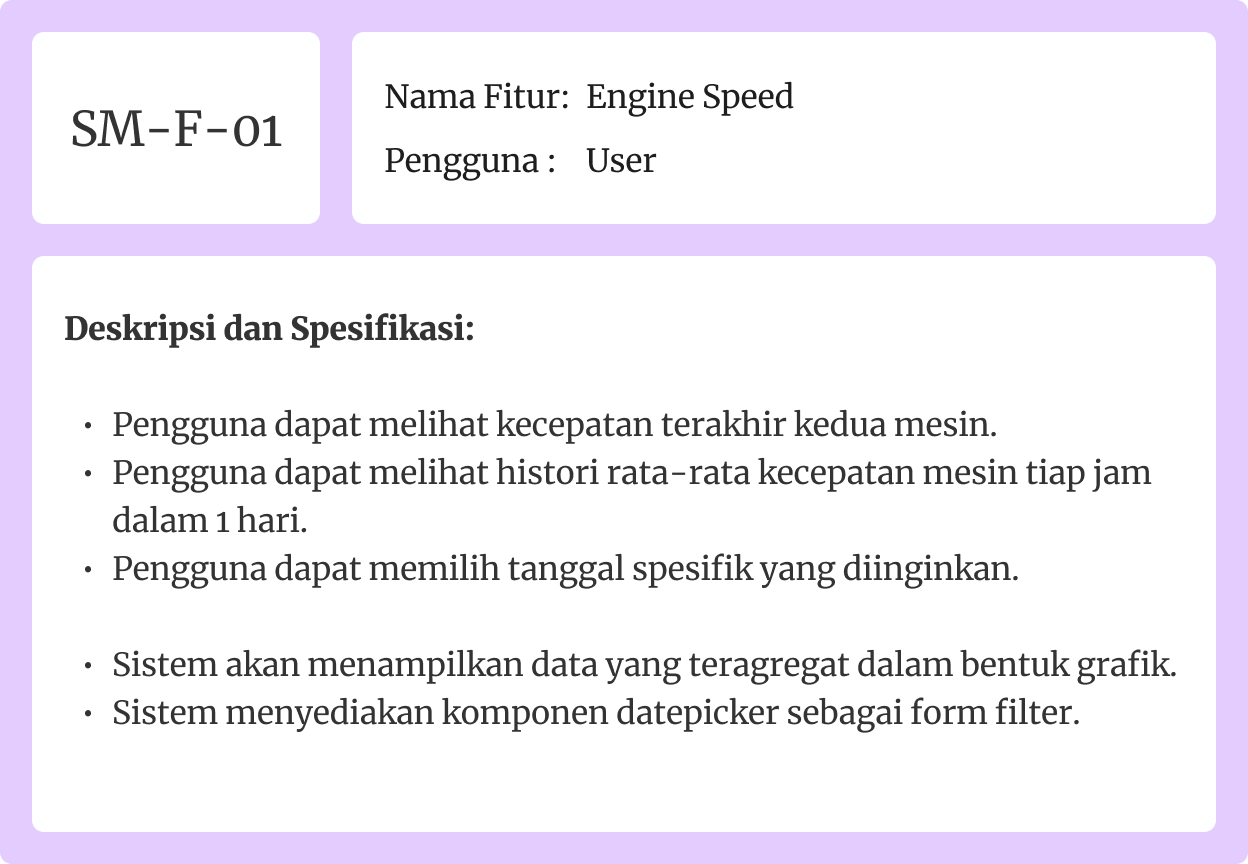
\includegraphics[width=.8\linewidth, center]{images/hasil/iterations/1/fr-es.png}
    \caption{Kebutuhan Fungsional Engine Speed}
    \label{fig:fr-es}
\end{figure}

\subsection{Desain}

Lalu, pada tahap desain dilakukan perancangan \textit{wireframe low fidelity} untuk memberikan gambaran pada pengembang terkait antar muka dari task yang dikerjakan. \textit{Wireframe} terdiri dari komponen dan tata letaknya tanpa teks atau konten detail.
Berikut merupakan desain \textit{wireframe} pada halaman Engine Speed. Pada halaman ini, pengguna dapat melihat angka kecepatan mesin terakhir dan nilai rata-rata dengan interval 1 jam dalam jangka waktu satu hari yang disajikan dalam bentuk grafik. Jangka waktu dapat dipilih melalui filter yang akan disediakan pada area komponen grafik. Seluruh navigasi pada sistem dapat dilakukan dengan memilih komponen \textit{Navbar} atau \textit{Sidebar}.

\begin{figure}[!h]
    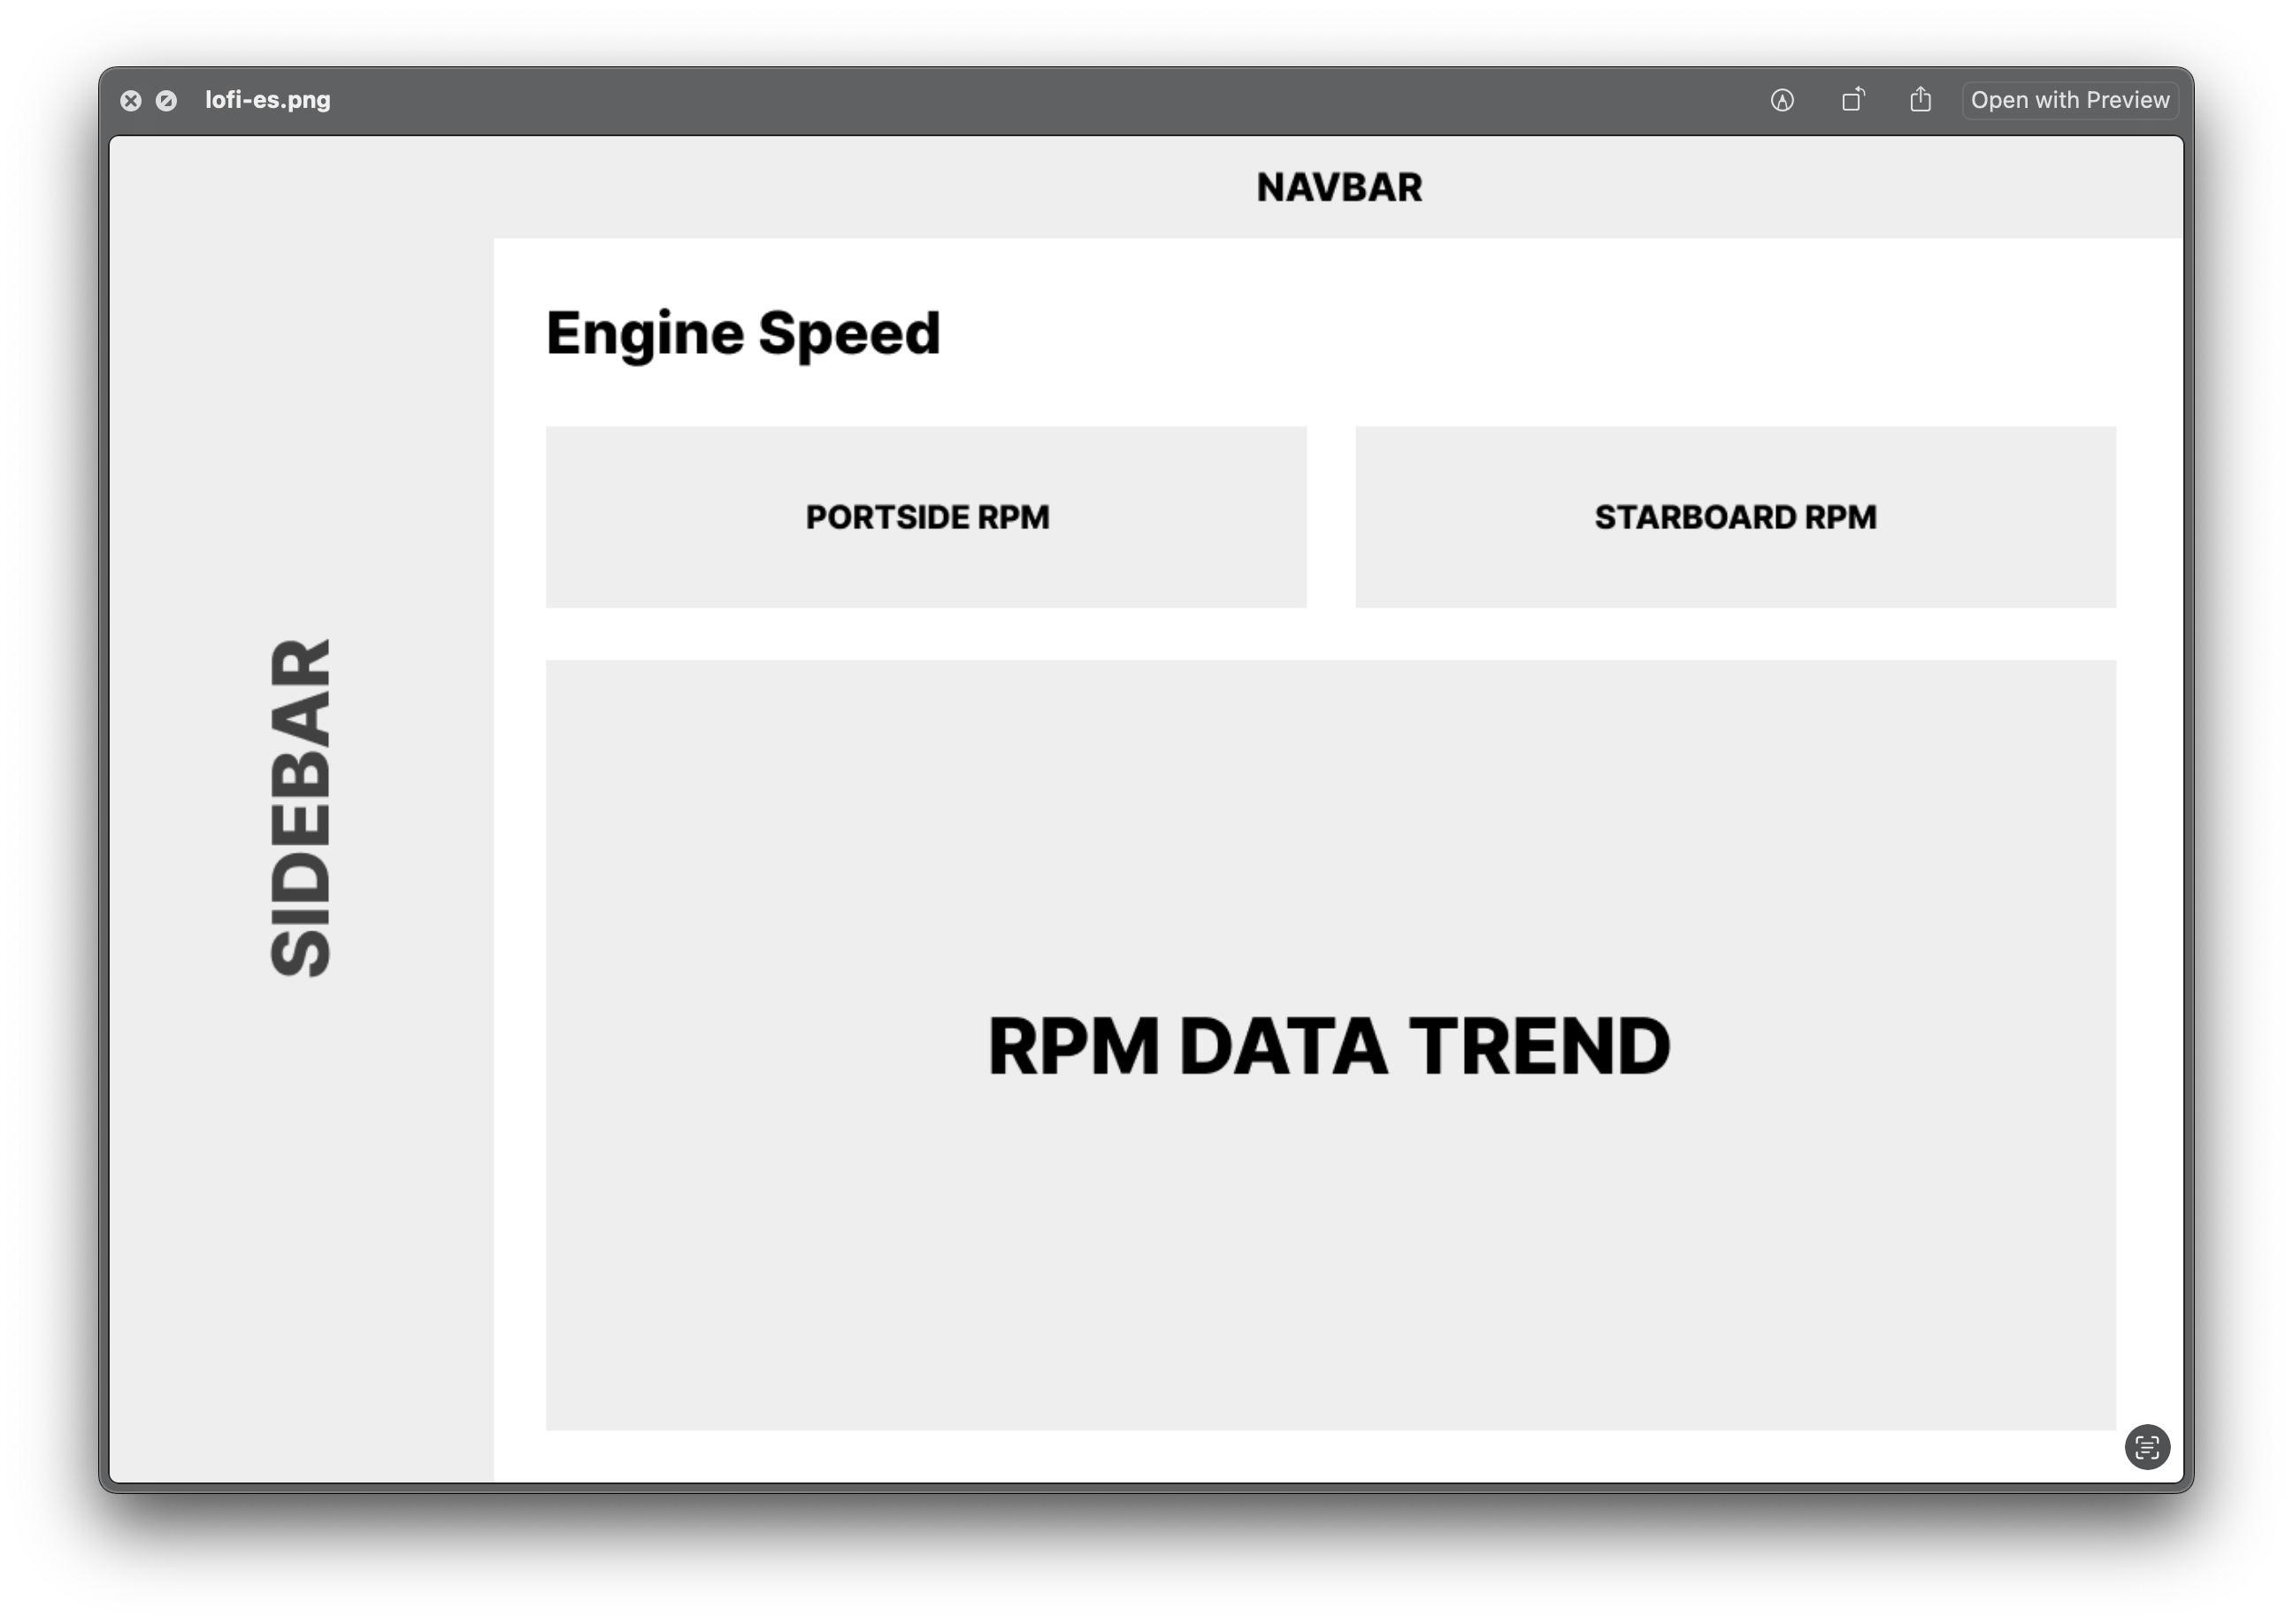
\includegraphics[width=1.05\linewidth, center]{images/hasil/iterations/1/lofi-es.png}
    \caption{\textit{Wireframe} Halaman Engine Speed}
    \label{fig:lofi-es}
\end{figure}

\subsection{Coding}

Berdasarkan desain low fidelity pada tahap desain maka dilakukan implementasi pengkodean tampilan halaman Engine Speed yang dapat dilihat pada Gambar \ref{fig:fe-es}. Halaman Engine Speed merupakan halaman untuk melihat kecepatan mesin terakhir dan histori tren dari kecepatan mesin yang disajikan dalam bentuk grafik garis. Pengguna dapat melakukan filter tanggal untuk mendapatkan data sesuai dengan batas waktu yang ditentukan.


\begin{figure}[!h]
    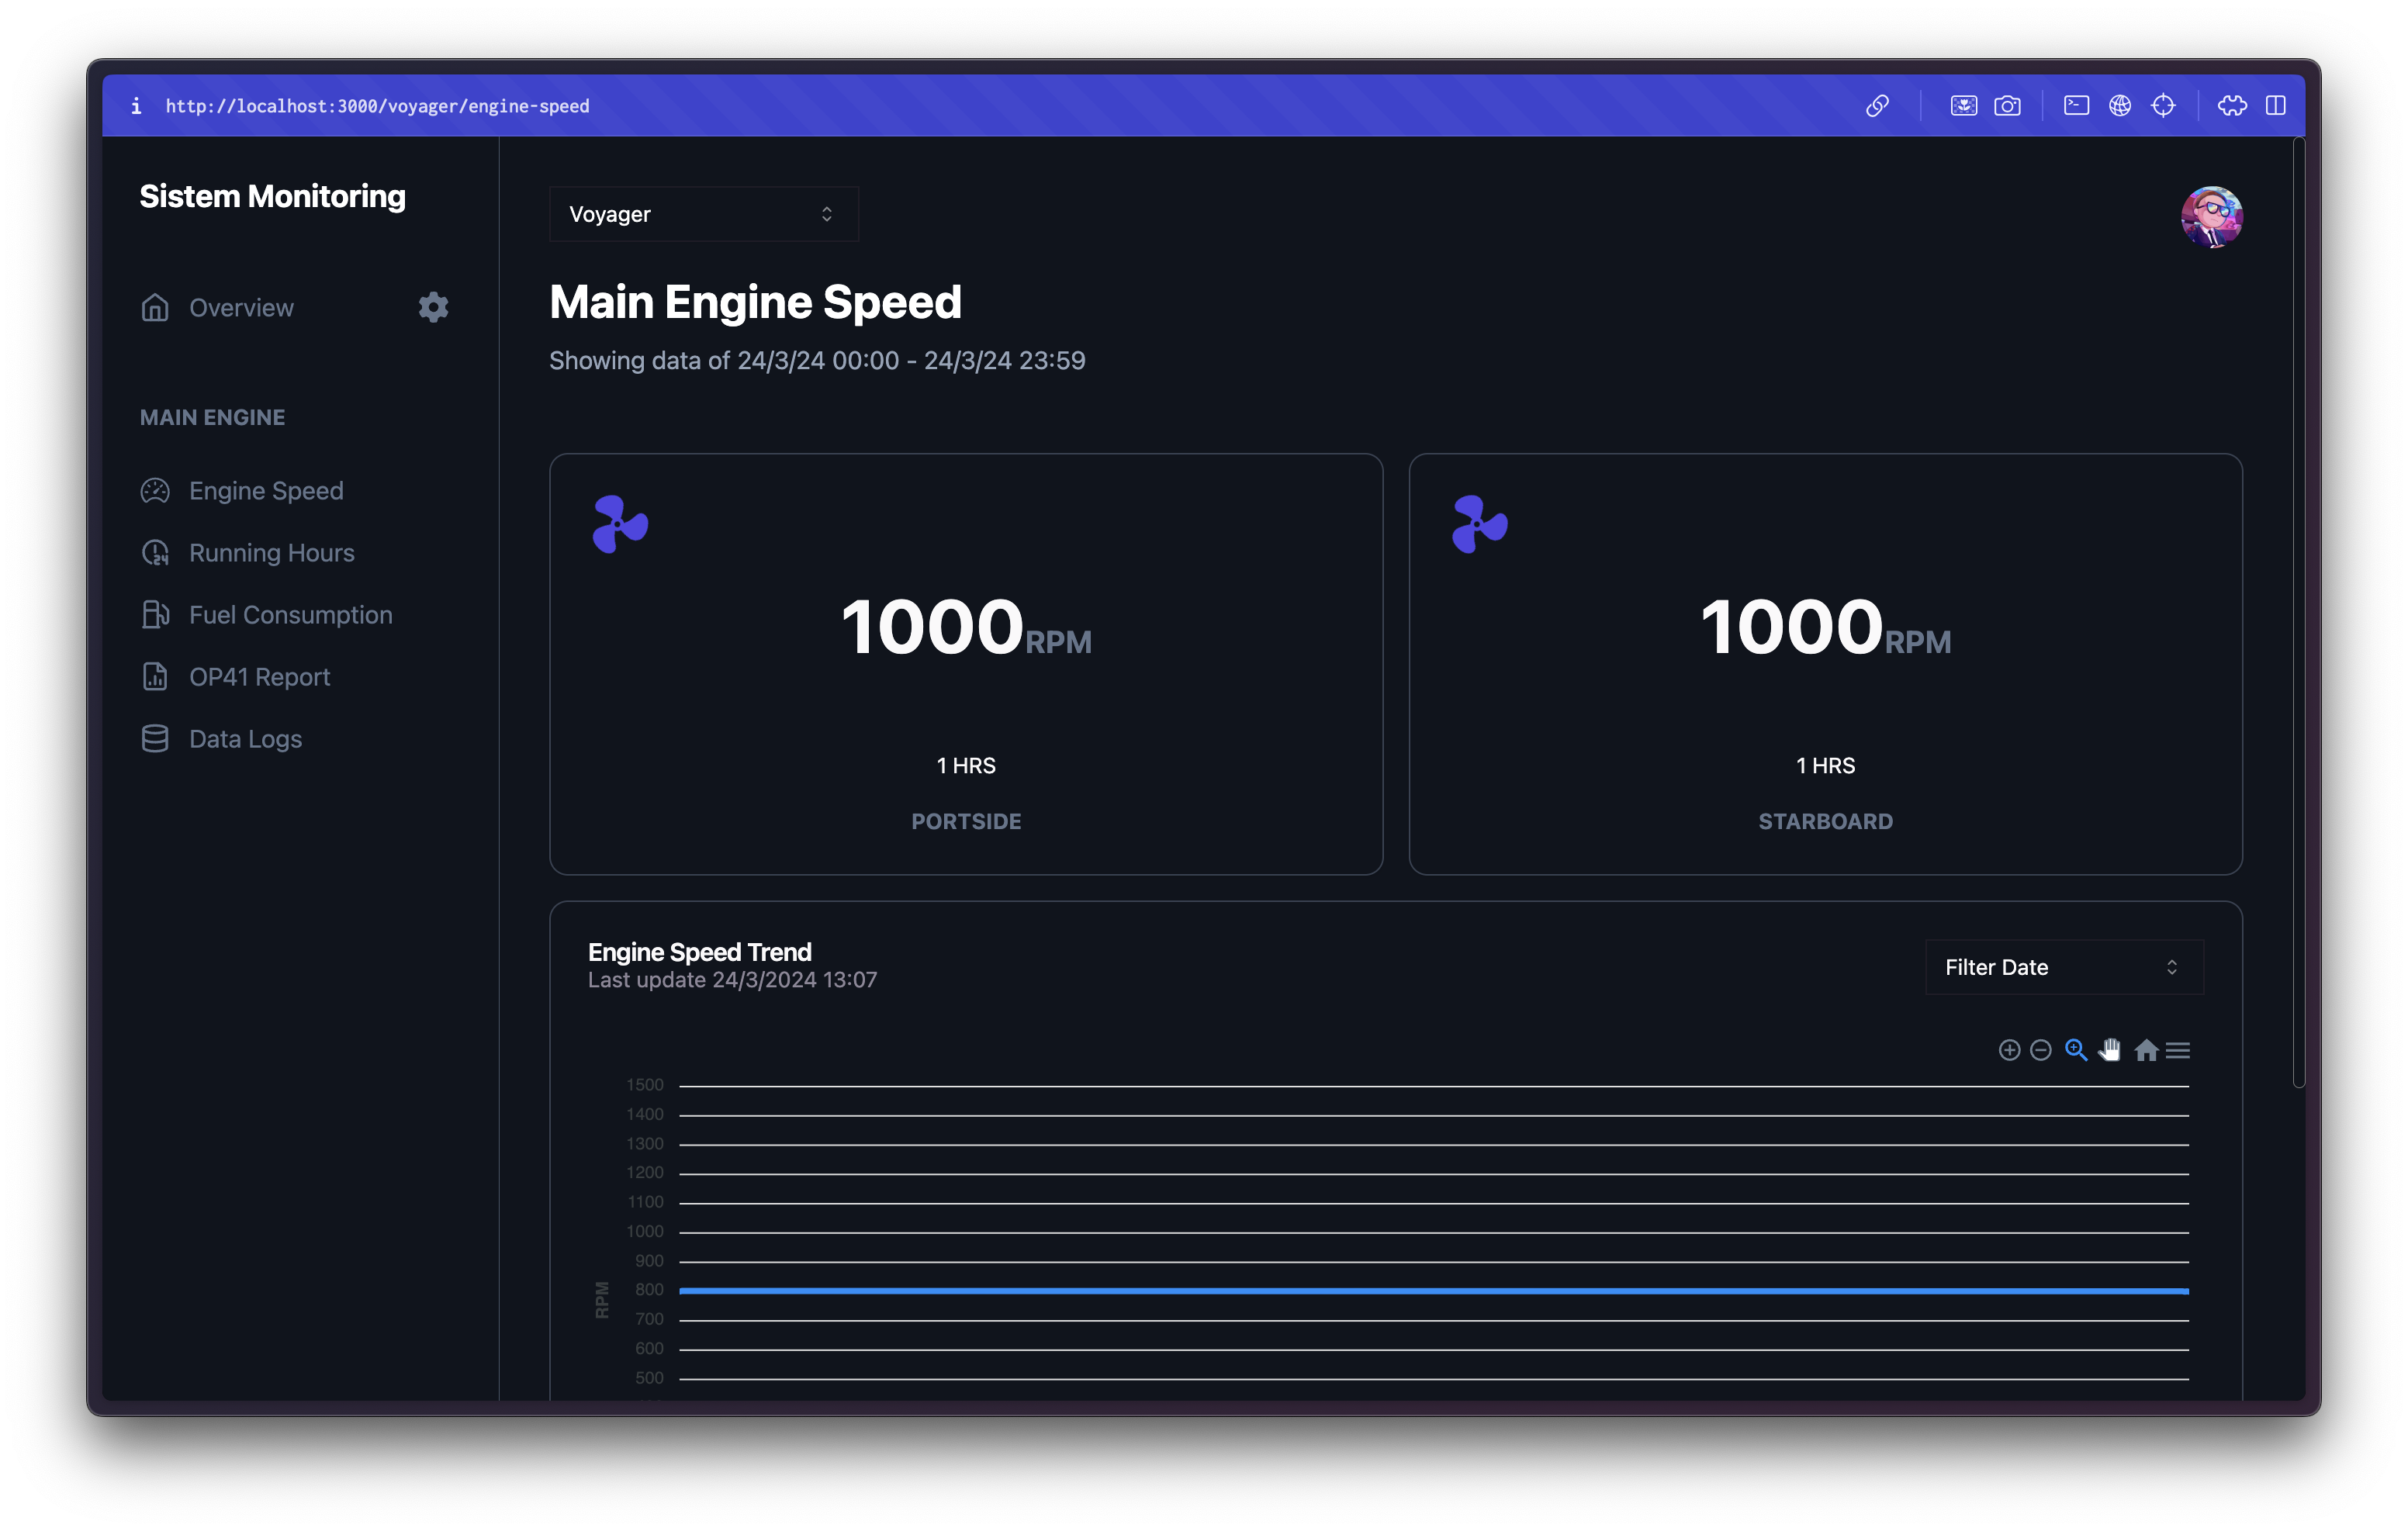
\includegraphics[width=1.05\linewidth, center]{images/hasil/iterations/1/fe-es.png}
    \caption{Frontend Halaman Engine Speed}
    \label{fig:fe-es}
\end{figure}

Halaman ini sepenuhnya menggunakan \textit{Client Side Rendering} (CSR). Hal ini memungkinkan pengguna untuk melakukan filter data tanpa perlu memuat ulang Halaman Engine Speed sehingga memaksimalkan pengalaman penggunaan sistem.

\subsection{Whitebox Testing}

Sebelum diunggah ke \textit{codebase} atau Github, dilakukan pengujian \textit{whitebox} dengan membuat \textit{Unit Test} yang akan dijalankan selama pengembangan. \textit{Unit test} dilakukan pada pengembagan API yang merupakan bagian dari \textit{Data Processing Layer} dan \textit{Network Layer}. Hal ini agar data yang akan ditampilkan pada antarmuka sistem merupakan data yang valid sehingga dapat memberikan wawasan yang tepat. \textit{Unit test} yang dibuat dapat dilihat pada Lampiran \ref{apdx:hasil}.

\begin{landscape}

    \subsection{Blackbox Testing}

    Setelah repositori telah terbarui, mitra dapat langsung mengakses sistem untuk menguji fungsionalitas fitur yang telah dikerjakan pada iterasi tersebut.

    \begin{table}[!h]
    \caption{Aturan Penomoran Blackbox Testing}
    \centering
    \begin{tabular}
        {
            >{\centering\arraybackslash}p{0.2\textwidth}
            >{\centering\arraybackslash}p{0.4\textwidth}
        }
        \toprule

        Kode &
        Keterangan \\ [1ex]

        \midrule

        SM- & Sistem Monitoring \\
        -T- & Testing \\
        -\{x\}- & Singkatan Nama Fitur \\
        -\{n\} & Nomor Urutan Test Case \\

        \bottomrule
    \end{tabular}
    \label{tab:nr-blackbox}
\end{table}

    \textit{Test case} yang dibuat untuk Halaman Engine Speed memastikan grafik telah ditampilkan dengan sesuai dan ketika pengguna melakukan filter tanggal, data grafik akan terubah sesuai dengan data tanggal yang diinput. Berikut hasil \textit{test case} untuk iterasi 1

    \begin{longtable}[!h]
    {
            p{0.2\textwidth}
            p{0.3\textwidth}
            p{0.3\textwidth}
            p{0.3\textwidth}
            p{0.3\textwidth}
            p{0.15\textwidth}
    }
    \caption{\textit{Blackbox Testing} Halaman Engine Speed}
    \label{tab:it1-blackbox-es} \\

    \hline
        \bfseries \textit{Test Code} &
        \bfseries \textit{Test Case} &
        \bfseries \textit{Test Steps} &
        \bfseries \textit{Expected Result} &
        \bfseries \textit{Actual Result} &
        \bfseries \textit{Pass/Fail} \\ [0.5ex]
    \hline

    \endfirsthead

    \hline
        \bfseries \textit{Test Code} &
        \bfseries \textit{Test Case} &
        \bfseries \textit{Test Steps} &
        \bfseries \textit{Expected Result} &
        \bfseries \textit{Actual Result} &
        \bfseries \textit{Pass/Fail} \\ [0.5ex]
    \hline
    \endhead % all the lines above this will be repeated on every page
    \hline

    \csvreader[
        late after line=\\,
        before reading={\catcode`\#=12},after reading={\catcode`\#=6}
    ]{tables/hasil/iterations/1/blackbox/engine-speed.csv}
    {1=\code, 2=\case, 3=\step, 4=\expect, 5=\actual, 6=\status}
    {\code & \case & \step & \expect & \actual & \status} \\

    \bottomrule
\end{longtable}
\end{landscape}

% Backup >?

% \begin{figure}[!h]
%     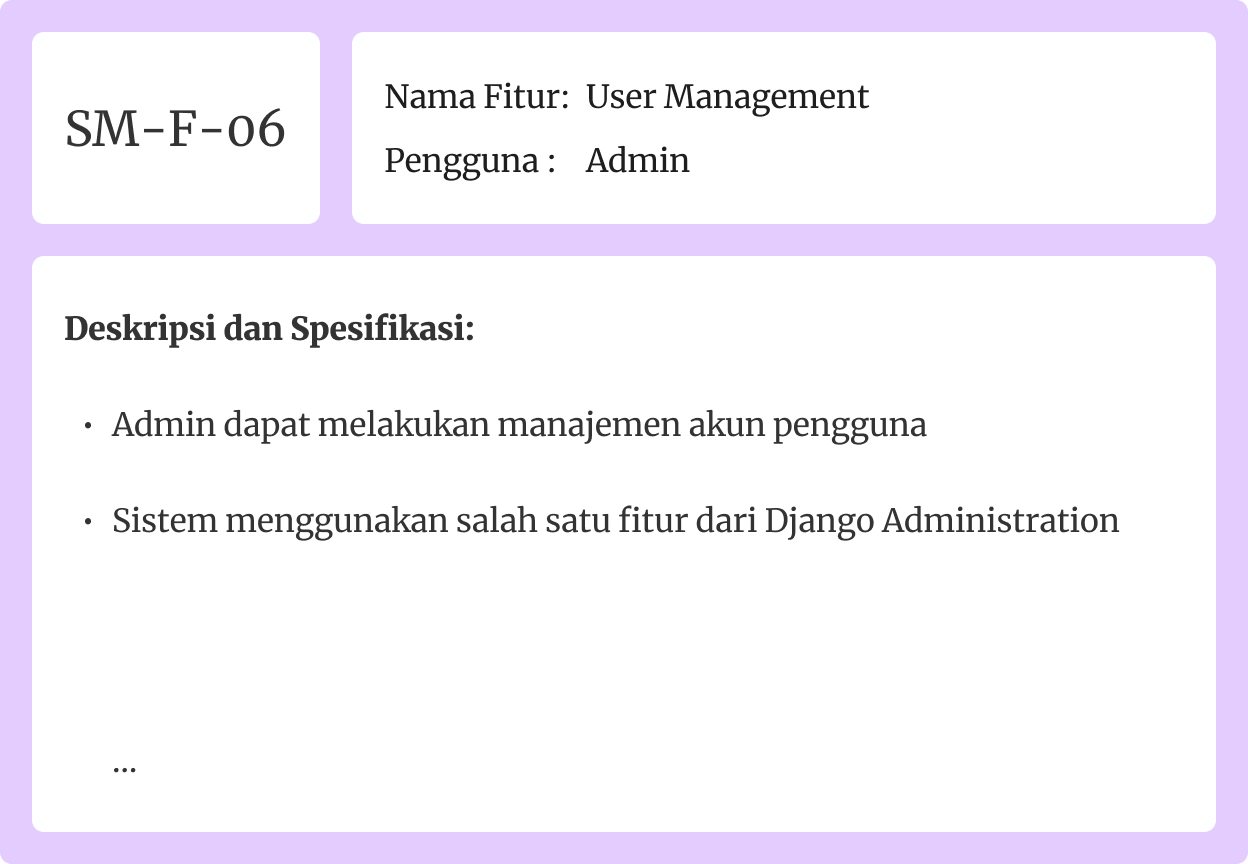
\includegraphics[width=.8\linewidth, center]{images/hasil/iterations/3/fr-user.png}
%     \caption{Kebutuhan Fungsional User Management}
%     \label{fig:fr-user}
% \end{figure}
% \begin{figure}[!h]
%     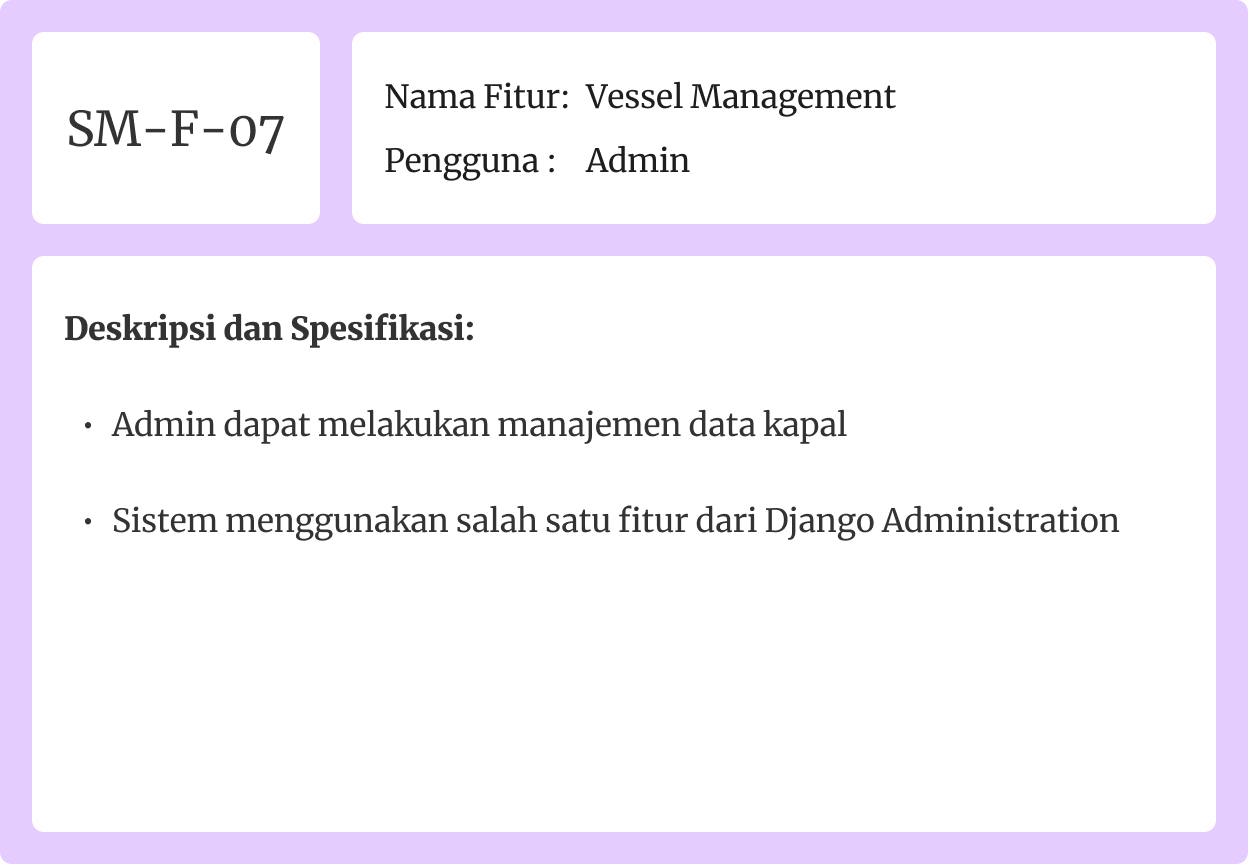
\includegraphics[width=.8\linewidth, center]{images/hasil/iterations/3/fr-vessel.png}
%     \caption{Kebutuhan Fungsional Vessel Management}
%     \label{fig:fr-vessel}
% \end{figure}
% \begin{figure}[!h]
%     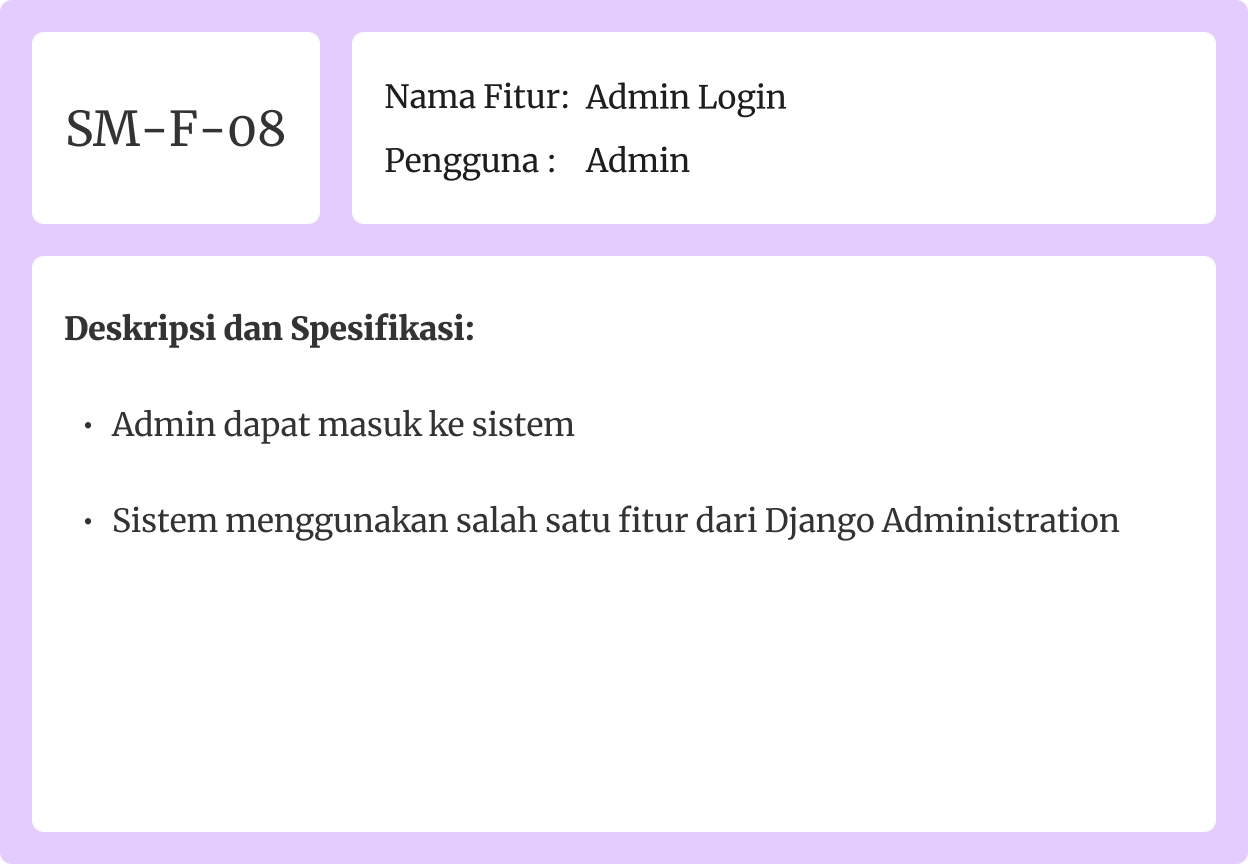
\includegraphics[width=.8\linewidth, center]{images/hasil/iterations/3/fr-login.png}
%     \caption{Kebutuhan Fungsional Admin Login}
%     \label{fig:fr-login-admin}
% \end{figure}

% \begin{figure}[!h]
%     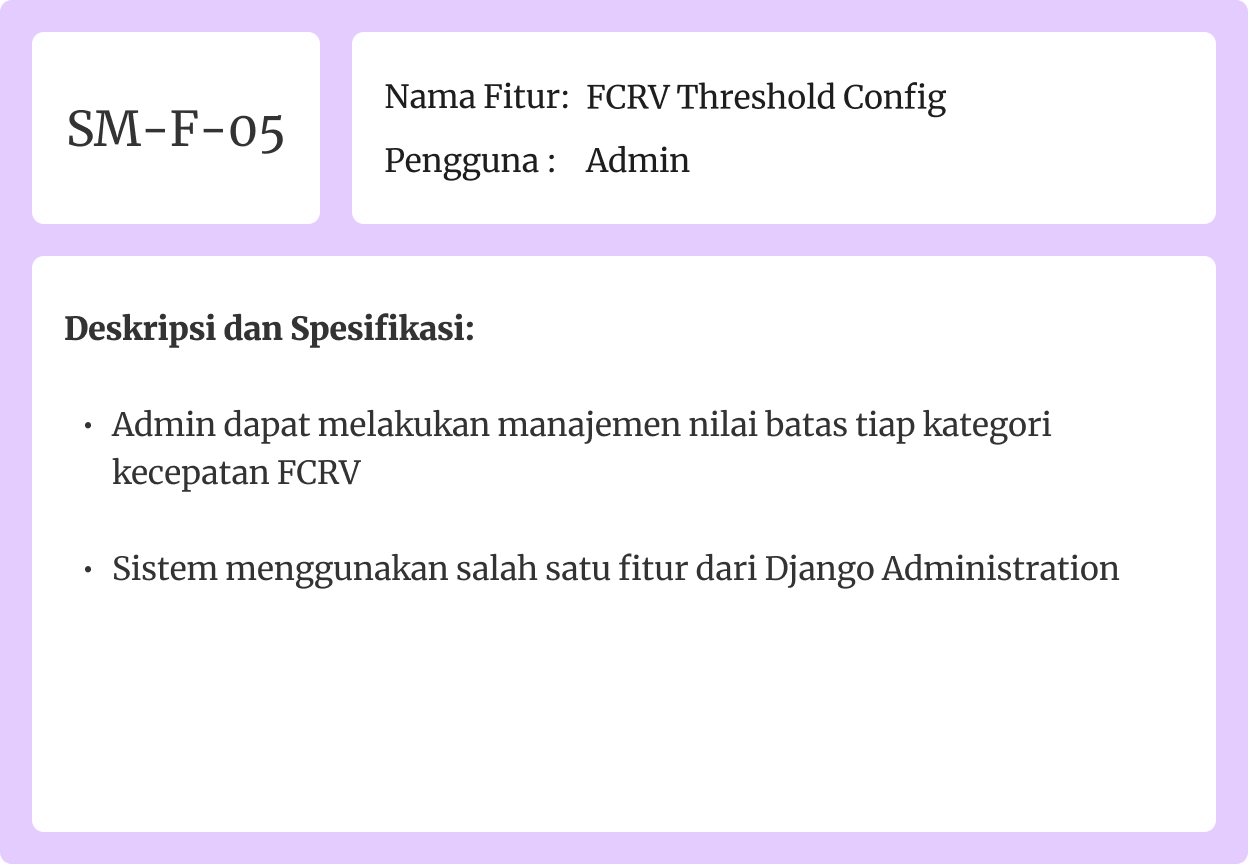
\includegraphics[width=.8\linewidth, center]{images/hasil/iterations/3/fr-fcrv.png}
%     \caption{Kebutuhan Fungsional Admin Logout}
%     \label{fig:fr-logout-admin}
% \end{figure}

% \newpage

% \subsubsection{Desain}

% Pada Sistem Admin, tidak dilakukan desain wireframe dikarenakan fitur bawaan framewok Django yang telah menyediakan Sistem Admin secara otomatis bernama Django administration.

% \subsubsection{Coding}

% Halaman Admin memungkinkan pengguna untuk melakukan operasi CRUD (create, read, update, dan delete) pada data pengguna, kapal, dan FCRV threshold. Hasil halaman yang dibuat oleh Django administration dapat dilihat pada Gambar ... hingga Gambar ... .

% \subsubsection{Whitebox Testing}

% Pada Django administration, seluruh komponen web dihasilkan oleh library bawaan dari package restapi yang telah diabstraksi sedemikian rupa dan telah memiliki alur pengujian sendiri. Sehingga, tidak dimungkinkan untuk dilakukan pengujian melalui unit test yang dibuat sendiri.

% \begin{landscape}
%     \subsubsection{Blackbox Testing}

%     \begin{longtable}[!h]
    {
            p{0.2\textwidth}
            p{0.3\textwidth}
            p{0.3\textwidth}
            p{0.3\textwidth}
            p{0.3\textwidth}
            p{0.15\textwidth}
    }
    \caption{Blackbox Testing Halaman User Management}
    \label{tab:it2-blackbox-user} \\

    \hline
        \bfseries \textit{Test Code} &
        \bfseries \textit{Test Case} &
        \bfseries \textit{Test Steps} &
        \bfseries \textit{Expected Result} &
        \bfseries \textit{Actual Result} &
        \bfseries \textit{Pass/Fail} \\ [0.5ex]
    \hline

    \endfirsthead

    \hline
        \bfseries \textit{Test Code} &
        \bfseries \textit{Test Case} &
        \bfseries \textit{Test Steps} &
        \bfseries \textit{Expected Result} &
        \bfseries \textit{Actual Result} &
        \bfseries \textit{Pass/Fail} \\ [0.5ex]
    \hline
    \endhead % all the lines above this will be repeated on every page
    \hline

    \csvreader[
        late after line=\\,
        before reading={\catcode`\#=12},after reading={\catcode`\#=6}
    ]{tables/hasil/iterations/3/blackbox/user.csv}
    {1=\code, 2=\case, 3=\step, 4=\expect, 5=\actual, 6=\status}
    {\code & \case & \step & \expect & \actual & \status} \\

    \bottomrule
\end{longtable}
%     \newpage
%     \begin{longtable}[!h]
    {
            p{0.2\textwidth}
            p{0.3\textwidth}
            p{0.3\textwidth}
            p{0.3\textwidth}
            p{0.3\textwidth}
            p{0.15\textwidth}
    }
    \caption{Blackbox Testing Halaman Vessel Management}
    \label{tab:it3-blackbox-vessel} \\

    \hline
        \bfseries \textit{Test Code} &
        \bfseries \textit{Test Case} &
        \bfseries \textit{Test Steps} &
        \bfseries \textit{Expected Result} &
        \bfseries \textit{Actual Result} &
        \bfseries \textit{Pass/Fail} \\ [0.5ex]
    \hline

    \endfirsthead

    \hline
        \bfseries \textit{Test Code} &
        \bfseries \textit{Test Case} &
        \bfseries \textit{Test Steps} &
        \bfseries \textit{Expected Result} &
        \bfseries \textit{Actual Result} &
        \bfseries \textit{Pass/Fail} \\ [0.5ex]
    \hline
    \endhead % all the lines above this will be repeated on every page
    \hline

    \csvreader[
        late after line=\\,
        before reading={\catcode`\#=12},after reading={\catcode`\#=6}
    ]{tables/hasil/iterations/3/blackbox/vessel.csv}
    {1=\code, 2=\case, 3=\step, 4=\expect, 5=\actual, 6=\status}
    {\code & \case & \step & \expect & \actual & \status} \\

    \bottomrule
\end{longtable}
%     \newpage
%     \begin{longtable}[!h]
    {
            p{0.2\textwidth}
            p{0.3\textwidth}
            p{0.3\textwidth}
            p{0.3\textwidth}
            p{0.3\textwidth}
            p{0.15\textwidth}
    }
    \caption{Blackbox Testing Halaman Autentikasi}
    \label{tab:it3-blackbox-auth-admin} \\

    \hline
        \bfseries \textit{Test Code} &
        \bfseries \textit{Test Case} &
        \bfseries \textit{Test Steps} &
        \bfseries \textit{Expected Result} &
        \bfseries \textit{Actual Result} &
        \bfseries \textit{Pass/Fail} \\ [0.5ex]
    \hline

    \endfirsthead

    \hline
        \bfseries \textit{Test Code} &
        \bfseries \textit{Test Case} &
        \bfseries \textit{Test Steps} &
        \bfseries \textit{Expected Result} &
        \bfseries \textit{Actual Result} &
        \bfseries \textit{Pass/Fail} \\ [0.5ex]
    \hline
    \endhead % all the lines above this will be repeated on every page
    \hline

    \csvreader[
        late after line=\\,
        before reading={\catcode`\#=12},after reading={\catcode`\#=6}
    ]{tables/hasil/iterations/3/blackbox/autentikasi.csv}
    {1=\code, 2=\case, 3=\step, 4=\expect, 5=\actual, 6=\status}
    {\code & \case & \step & \expect & \actual & \status} \\

    \bottomrule
\end{longtable}
% \end{landscape}

% \subsection{Iterasi 4}

% \subsubsection{Analisis}

% Pada iterasi 4, difokuskan untuk membuat fitur spesifik seperti membuat laporan kecepatan mesin harian dan laporan konsumsi bahan bakar harian yang secara berturut-turut terdapat pada Halaman Engine Speed dan Fuel Consumption. Kebutuhan fungsional dapat dilihat pada Gambar \ref{fig:fr-generate-es-report} dan Gambar \ref{fig:fr-generate-fuel-report}.

% \begin{figure}[!h]
%     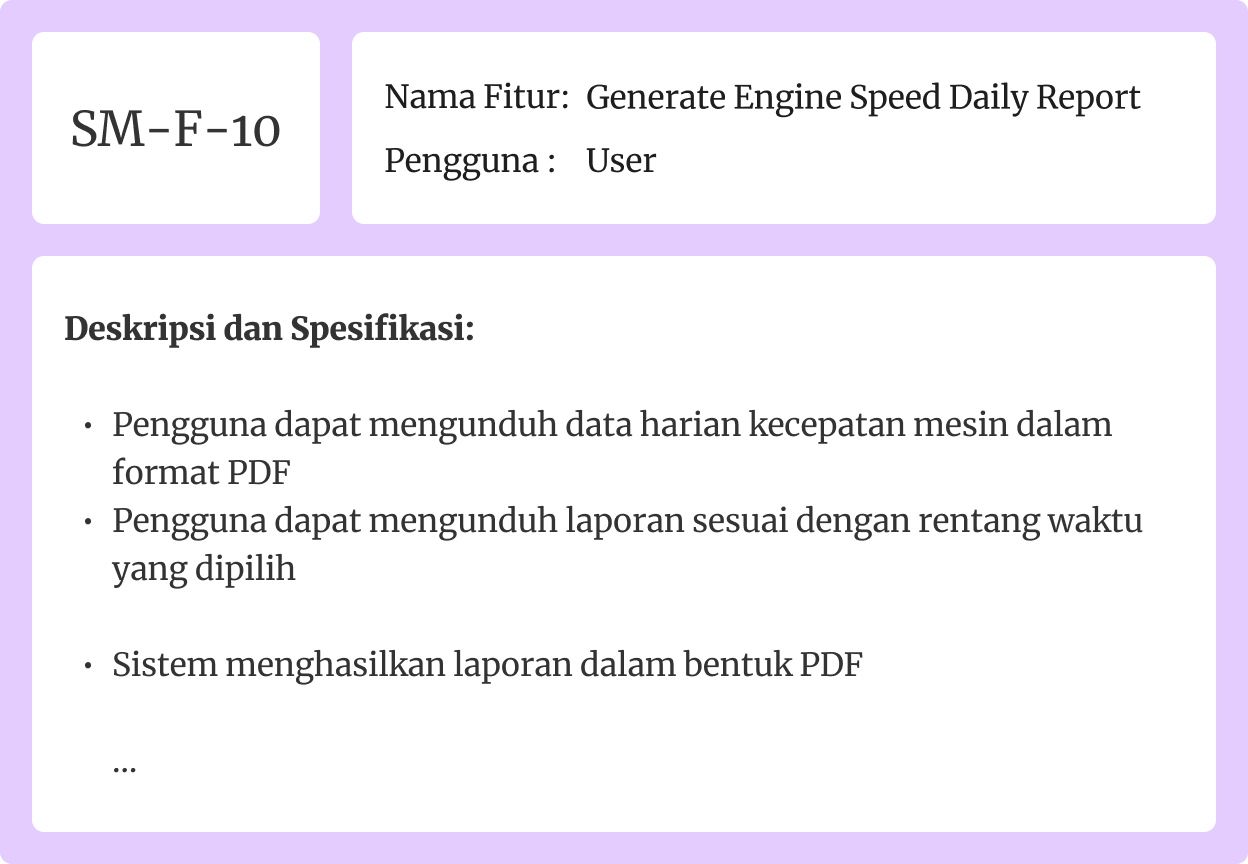
\includegraphics[width=.8\linewidth, center]{images/hasil/iterations/4/fr-generate-es-report.png}
%     \caption{Kebutuhan Fungsional Generate Engine Speed Daily Report}
%     \label{fig:fr-generate-es-report}
% \end{figure}

% \begin{figure}[!h]
%     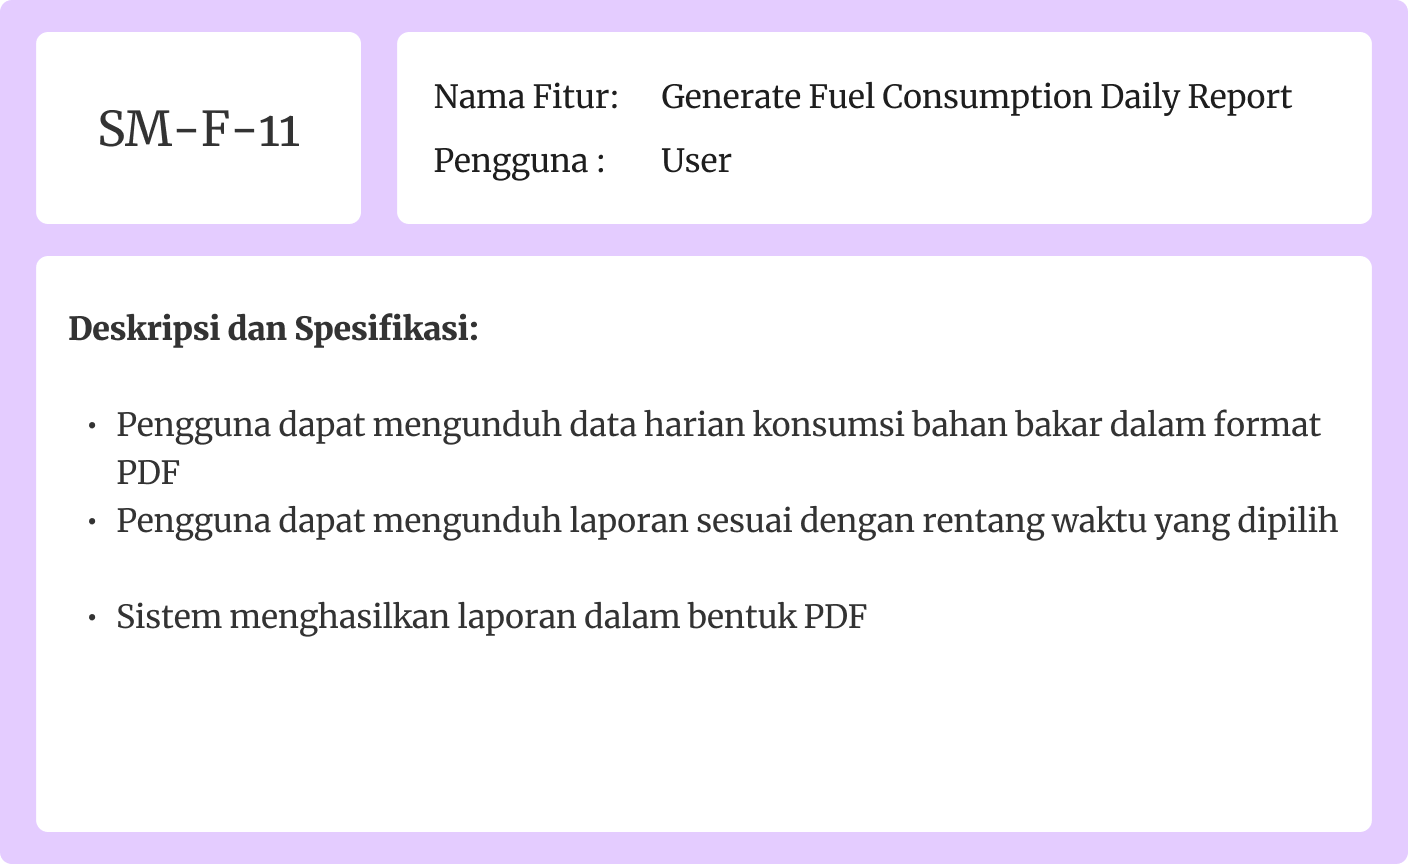
\includegraphics[width=.8\linewidth, center]{images/hasil/iterations/4/fr-generate-fuel-report.png}
%     \caption{Kebutuhan Fungsional Generate Fuel Consumption Daily Report}
%     \label{fig:fr-generate-fuel-report}
% \end{figure}

% \subsubsection{Desain}

% Pada tahap ini, dilakukan desain laporan bahan bakar yang kemudian dapat dibuat secara dinamis oleh sistem. Laporan kecepatan mesin dan bahan bakar dapat dilihat pada Gambar \ref{fig:es-report} dan Gambar \ref{fig:fc-report}.

% \begin{figure}[!h]
%     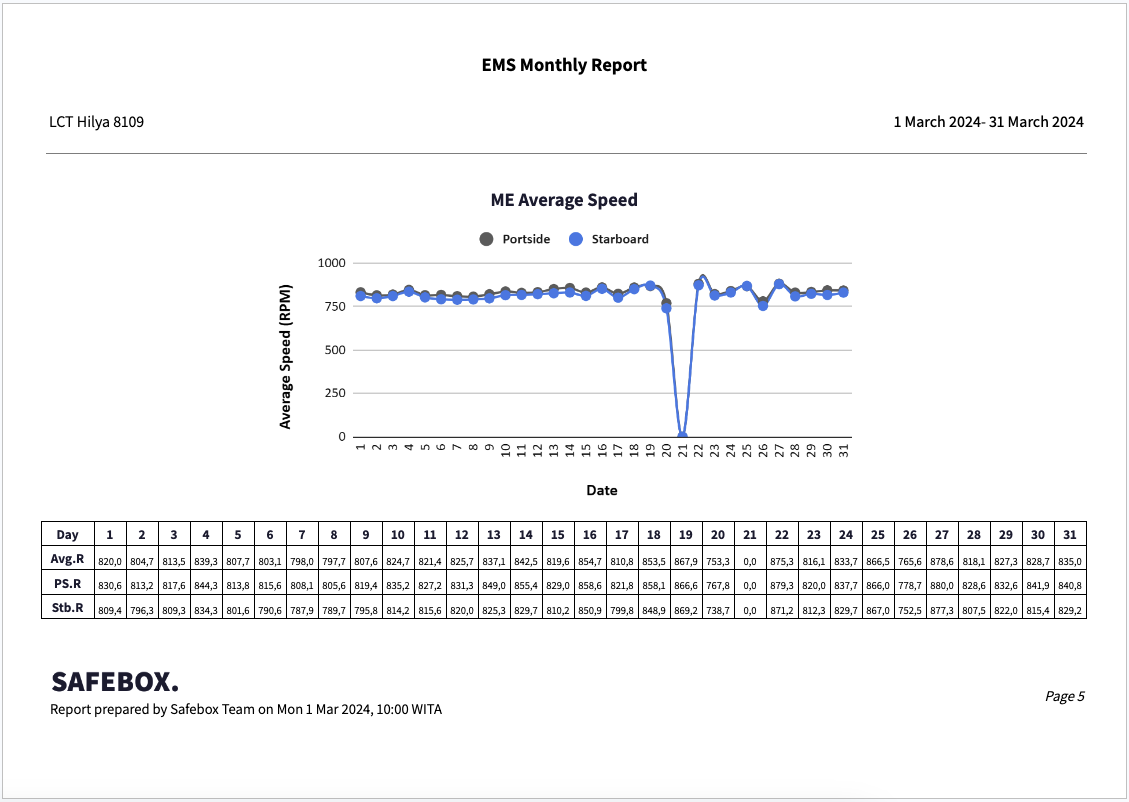
\includegraphics[width=1\linewidth, center]{images/hasil/iterations/4/es-report.png}
%     \caption{Contoh Laporan Kecepatan Mesin}
%     \label{fig:es-report}
% \end{figure}

% \begin{figure}[!h]
%     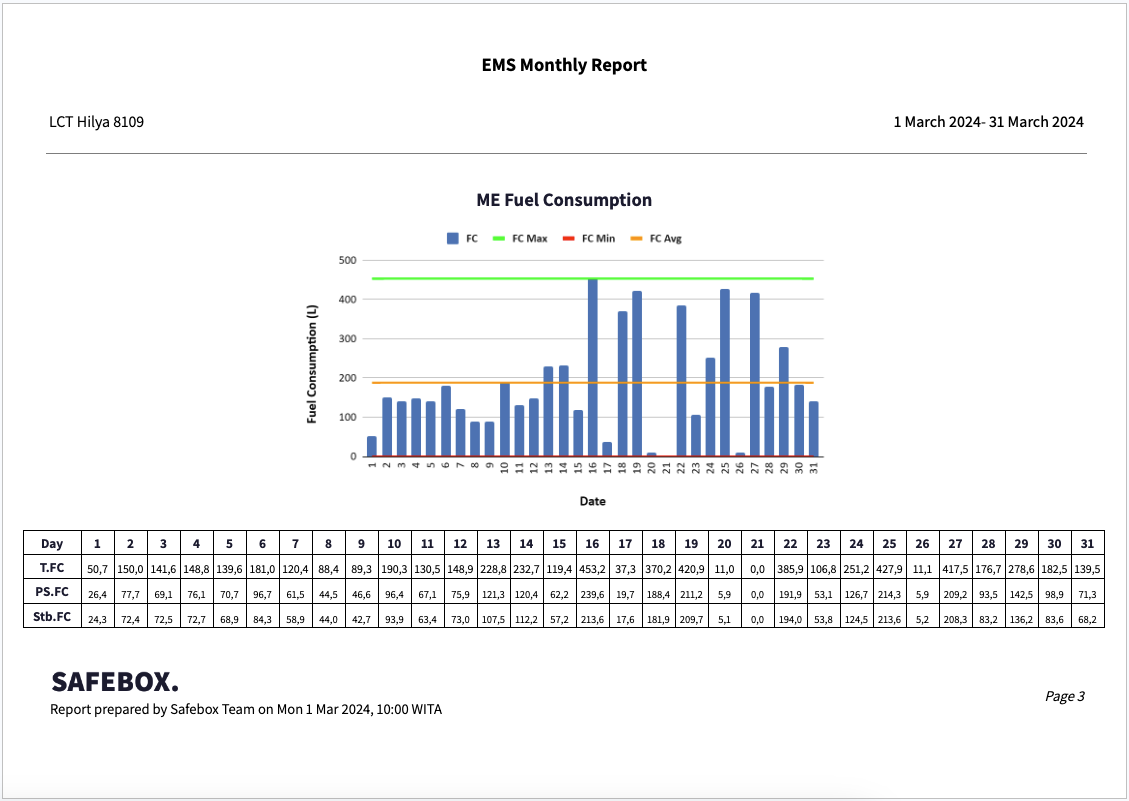
\includegraphics[width=1\linewidth, center]{images/hasil/iterations/4/fc-report.png}
%     \caption{Contoh Laporan Konsumsi Bahan Bakar}
%     \label{fig:fc-report}
% \end{figure}

% \newpage

% \subsubsection{Coding}
% \subsubsection{Whitebox Testing}

% \begin{landscape}
%     \subsubsection{Blackbox Testing}

%     \begin{longtable}[!h]
    {
            p{0.2\textwidth}
            p{0.3\textwidth}
            p{0.3\textwidth}
            p{0.3\textwidth}
            p{0.3\textwidth}
            p{0.15\textwidth}
    }
    \caption{\textit{Blackbox Testing Generate Engine Speed Daily Report}}
    \label{tab:it4-blackbox-generate-es-report} \\

    \hline
        \bfseries \textit{Test Code} &
        \bfseries \textit{Test Case} &
        \bfseries \textit{Test Steps} &
        \bfseries \textit{Expected Result} &
        \bfseries \textit{Actual Result} &
        \bfseries \textit{Pass/Fail} \\ [0.5ex]
    \hline

    \endfirsthead

    \hline
        \bfseries \textit{Test Code} &
        \bfseries \textit{Test Case} &
        \bfseries \textit{Test Steps} &
        \bfseries \textit{Expected Result} &
        \bfseries \textit{Actual Result} &
        \bfseries \textit{Pass/Fail} \\ [0.5ex]
    \hline
    \endhead % all the lines above this will be repeated on every page
    \hline

    \csvreader[
        late after line=\\,
        before reading={\catcode`\#=12},after reading={\catcode`\#=6}
    ]{tables/hasil/iterations/4/blackbox/generate-es-report.csv}
    {1=\code, 2=\case, 3=\step, 4=\expect, 5=\actual, 6=\status}
    {\code & \case & \step & \expect & \actual & \status} \\

    \bottomrule
\end{longtable}
%     \newpage
%     \begin{longtable}[!h]
    {
            p{0.2\textwidth}
            p{0.3\textwidth}
            p{0.3\textwidth}
            p{0.3\textwidth}
            p{0.3\textwidth}
            p{0.15\textwidth}
    }
    \caption{\textit{Blackbox Testing Generate Fuel Consumption Daily Report}}
    \label{tab:it4-blackbox-generate-fuel-report} \\

    \hline
        \bfseries \textit{Test Code} &
        \bfseries \textit{Test Case} &
        \bfseries \textit{Test Steps} &
        \bfseries \textit{Expected Result} &
        \bfseries \textit{Actual Result} &
        \bfseries \textit{Pass/Fail} \\ [0.5ex]
    \hline

    \endfirsthead

    \hline
        \bfseries \textit{Test Code} &
        \bfseries \textit{Test Case} &
        \bfseries \textit{Test Steps} &
        \bfseries \textit{Expected Result} &
        \bfseries \textit{Actual Result} &
        \bfseries \textit{Pass/Fail} \\ [0.5ex]
    \hline
    \endhead % all the lines above this will be repeated on every page
    \hline

    \csvreader[
        late after line=\\,
        before reading={\catcode`\#=12},after reading={\catcode`\#=6}
    ]{tables/hasil/iterations/4/blackbox/generate-fuel-report.csv}
    {1=\code, 2=\case, 3=\step, 4=\expect, 5=\actual, 6=\status}
    {\code & \case & \step & \expect & \actual & \status} \\

    \bottomrule
\end{longtable}
% \end{landscape}

% \subsection{Iterasi 5}

% \subsubsection{Analisis}

% Pada iterasi terakhir, dilakukan pengembangan fitur ekspor data yang terdapat pada Halaman Data Log, autentikasi sistem, Halaman OP41 Report, dan Halaman Overview. Kebutuhan fungsional dapat dilihat pada Gambar \ref{fig:fr-export-data} hingga Gambar \ref{fig:fr-op41}

% \begin{figure}[!h]
%     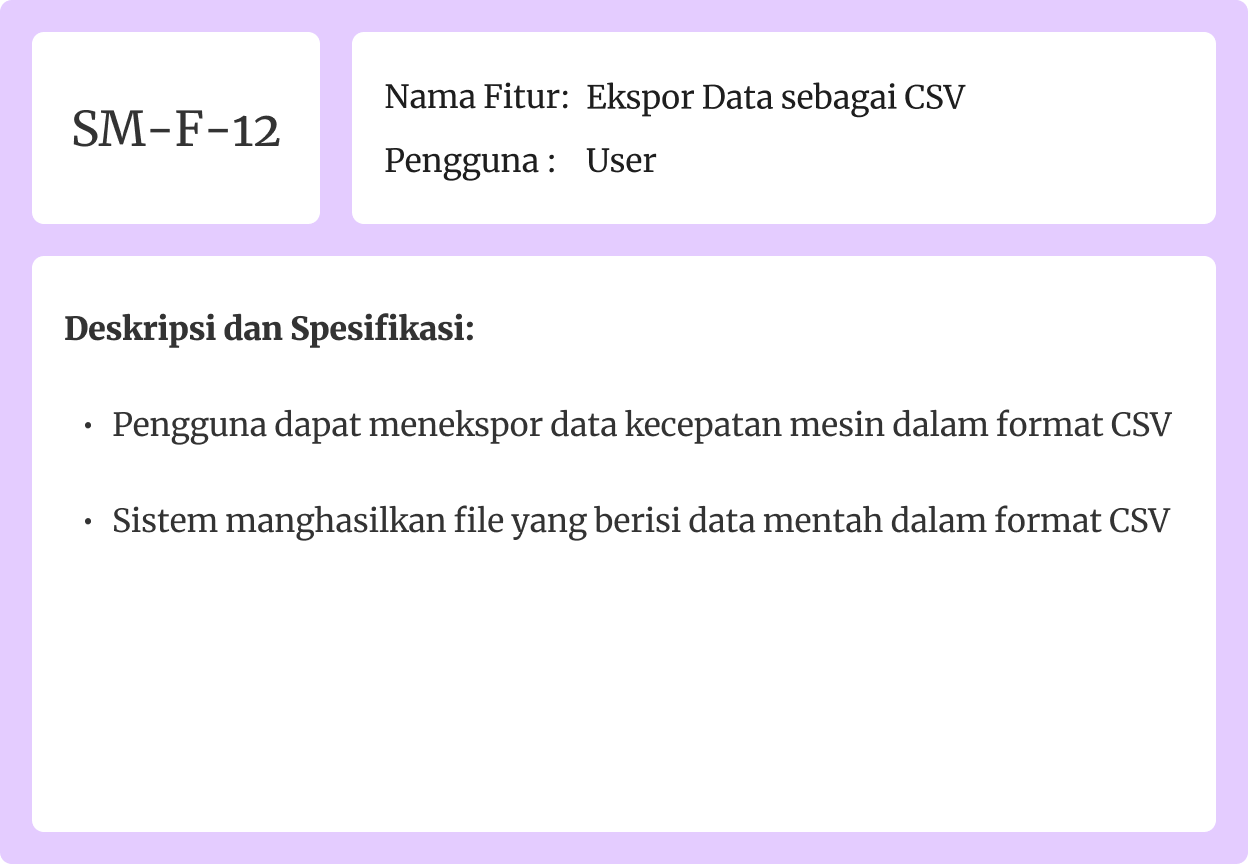
\includegraphics[width=1\linewidth, center]{images/hasil/iterations/5/fr-export-data.png}
%     \caption{Kebutuhan Fungsional Ekspor Data}
%     \label{fig:fr-export-data}
% \end{figure}

% \begin{figure}[!h]
%     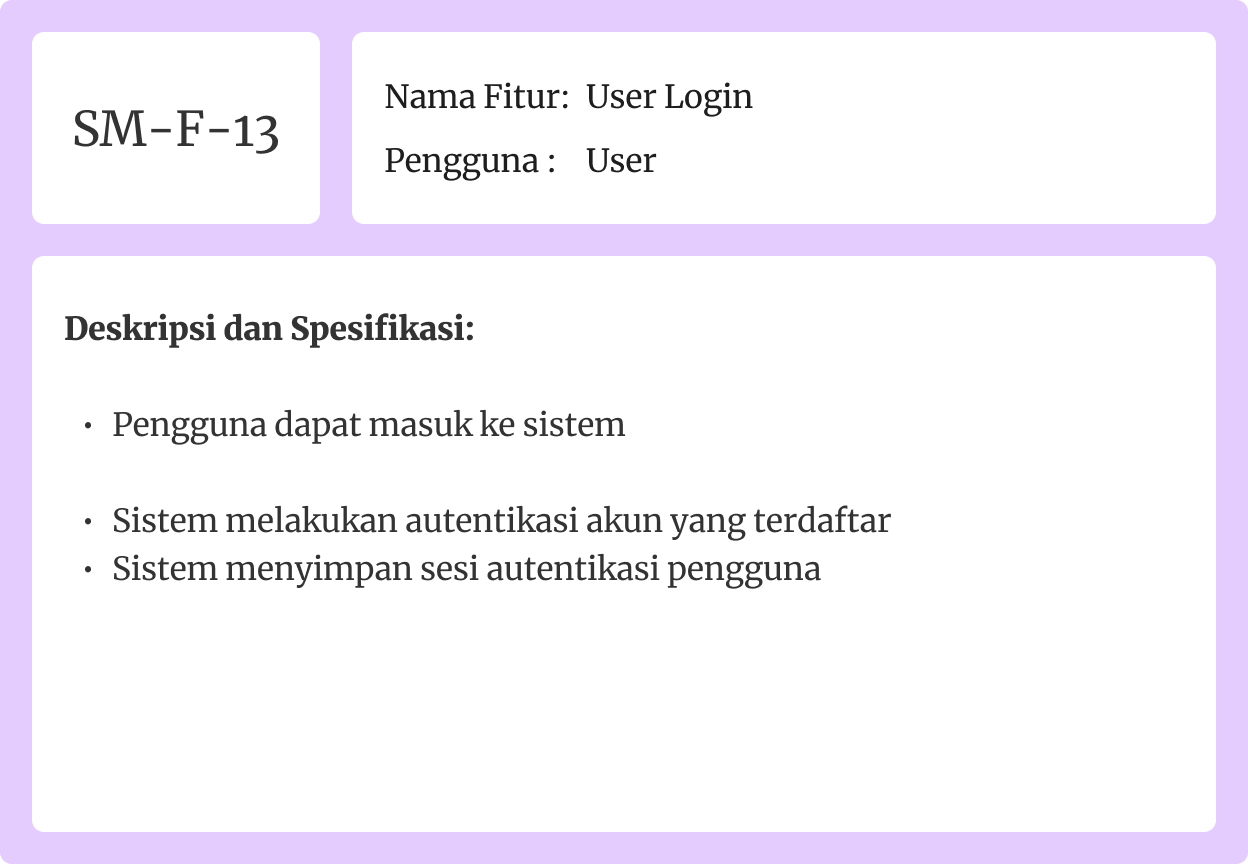
\includegraphics[width=1\linewidth, center]{images/hasil/iterations/5/fr-login-user.png}
%     \caption{Kebutuhan Fungsional User Login}
%     \label{fig:fr-login-user}
% \end{figure}

% \begin{figure}[!h]
%     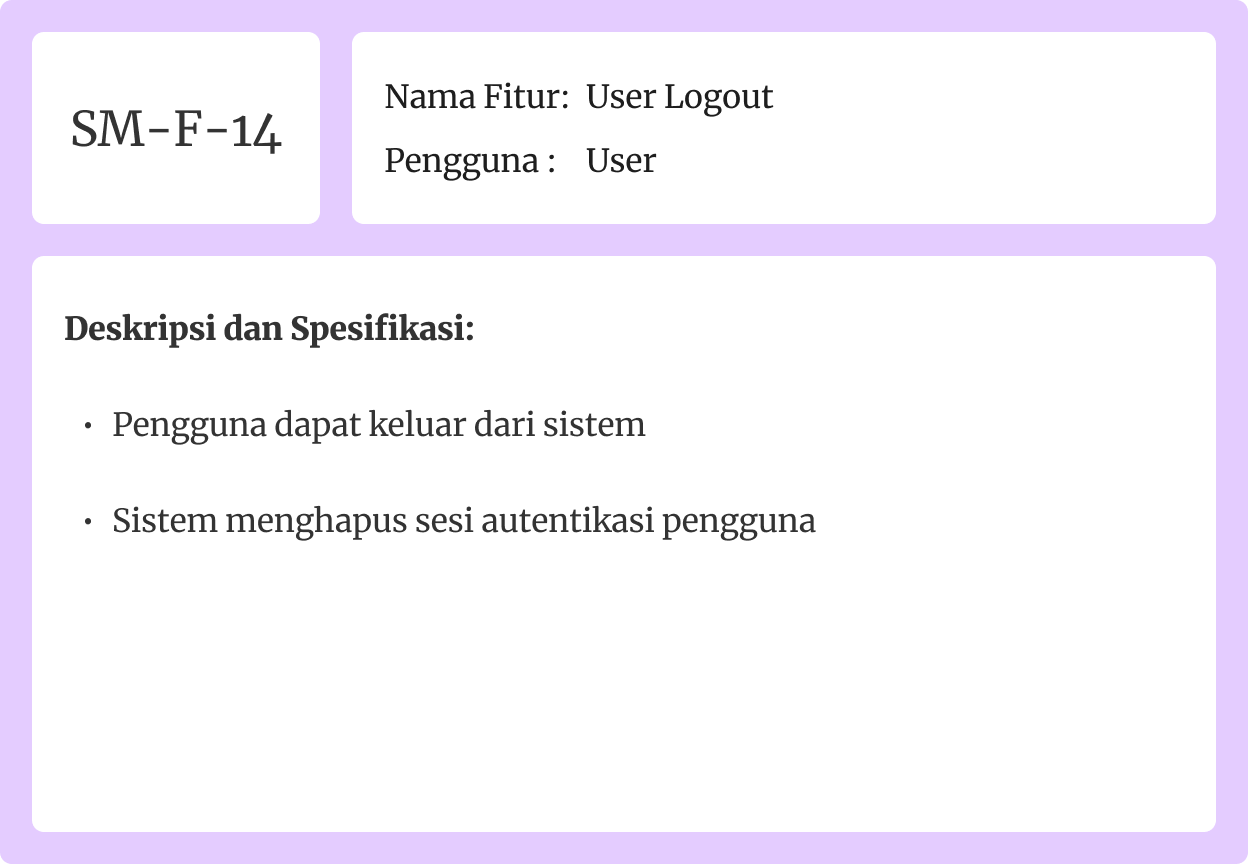
\includegraphics[width=1\linewidth, center]{images/hasil/iterations/5/fr-logout-user.png}
%     \caption{Kebutuhan Fungsional User Logout}
%     \label{fig:fr-logout-user}
% \end{figure}

% \begin{figure}[!h]
%     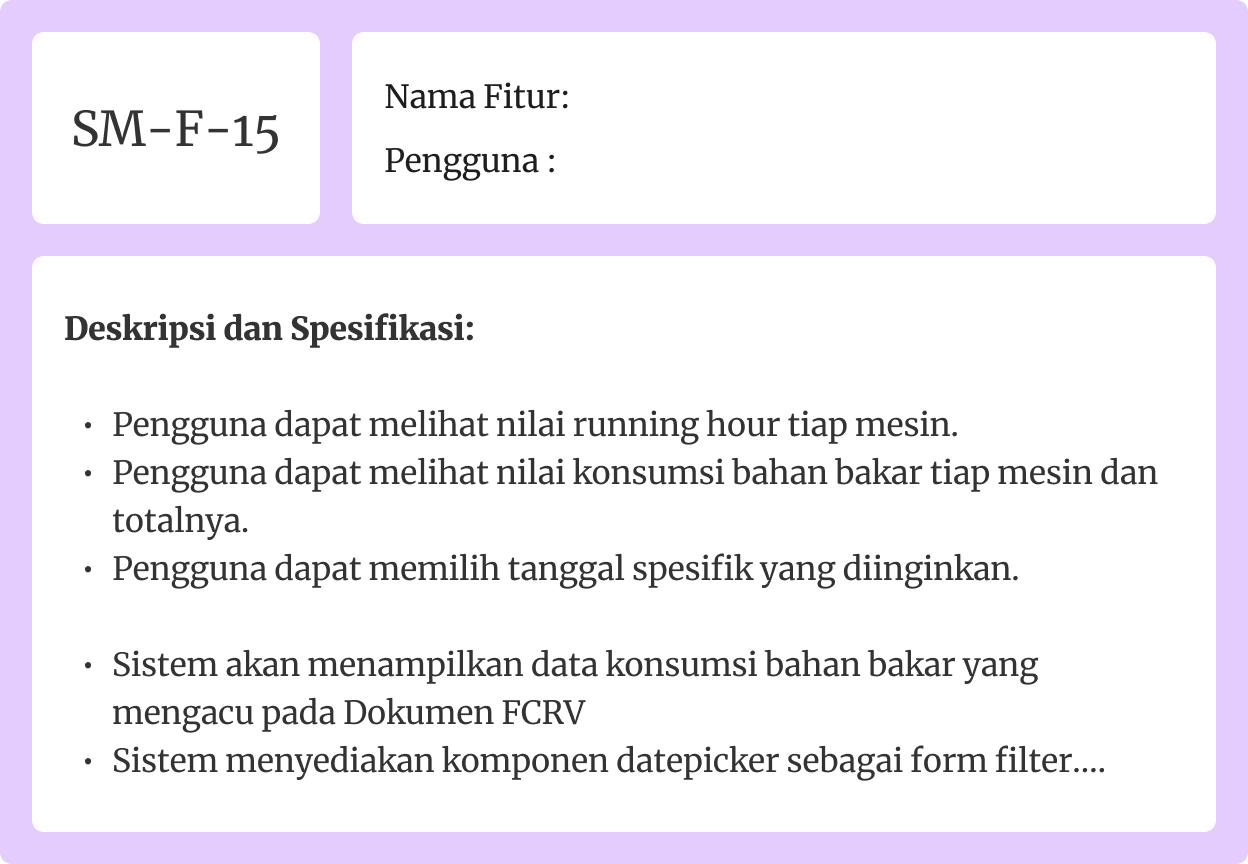
\includegraphics[width=1\linewidth, center]{images/hasil/iterations/5/fr-op41.png}
%     \caption{Kebutuhan Fungsional OP41 Report}
%     \label{fig:fr-op41}
% \end{figure}

% \newpage

% \subsubsection{Desain}

% Dilakukan desain pada Halaman Login, OP41 Report, dan Overview yang dapat dilihat pada Gambar \ref{fig:lofi-login}, Gambar \ref{fig:lofi-op41} dan Gambar \ref{lif-} secara berturut-turut.

% \begin{figure}[!h]
%     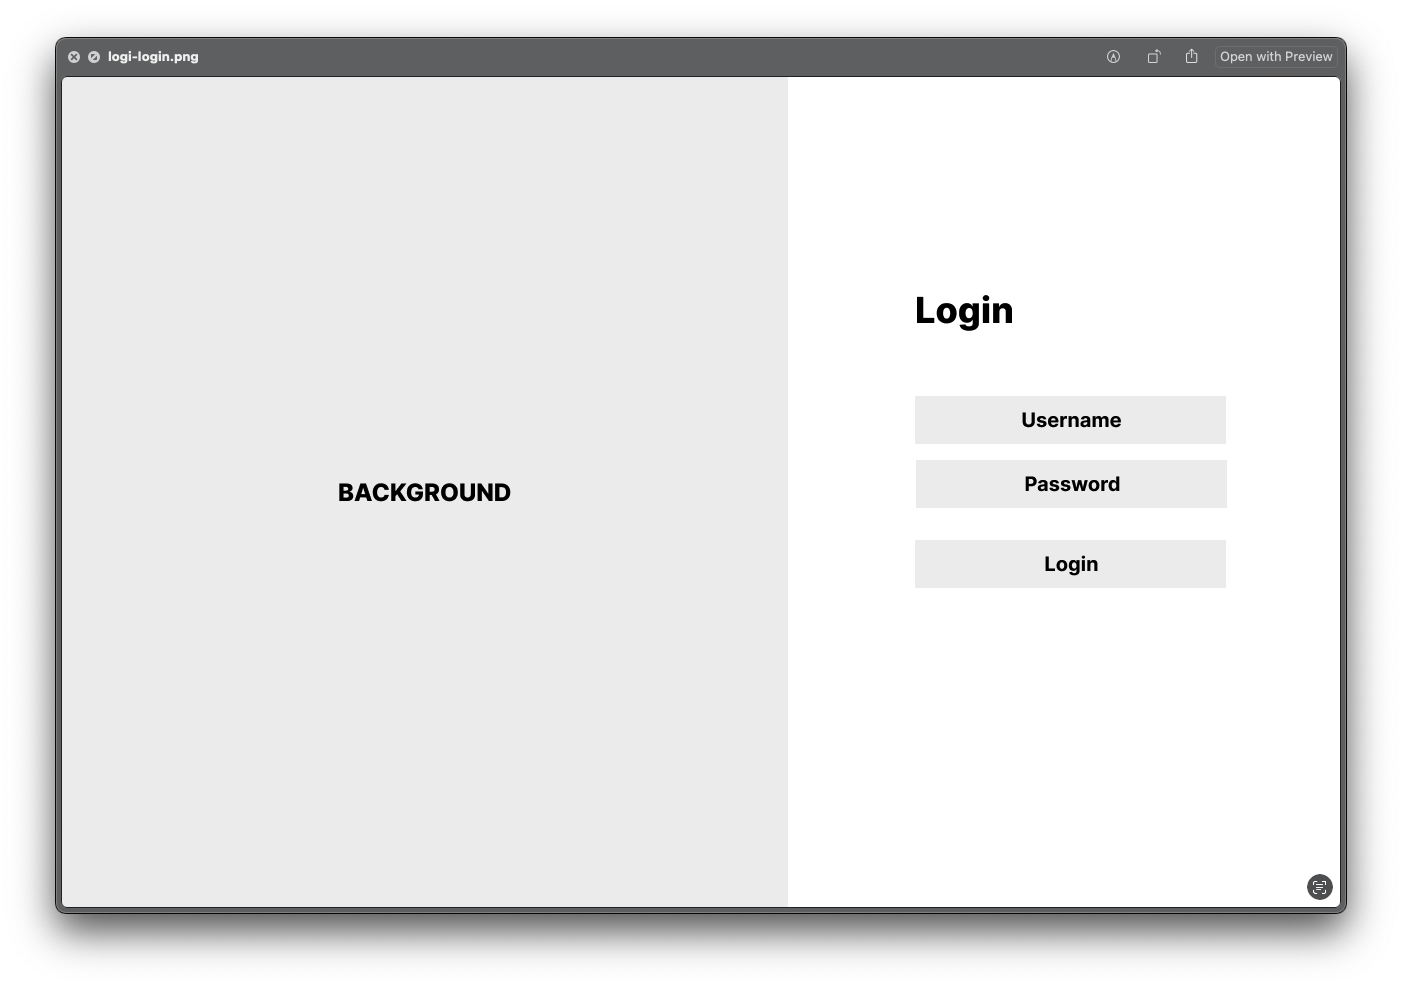
\includegraphics[width=1.05\linewidth, center]{images/hasil/iterations/5/lofi-login.png}
%     \caption{Wireframe Halaman Login}
%     \label{fig:lofi-login}
% \end{figure}

% \begin{figure}[!h]
%     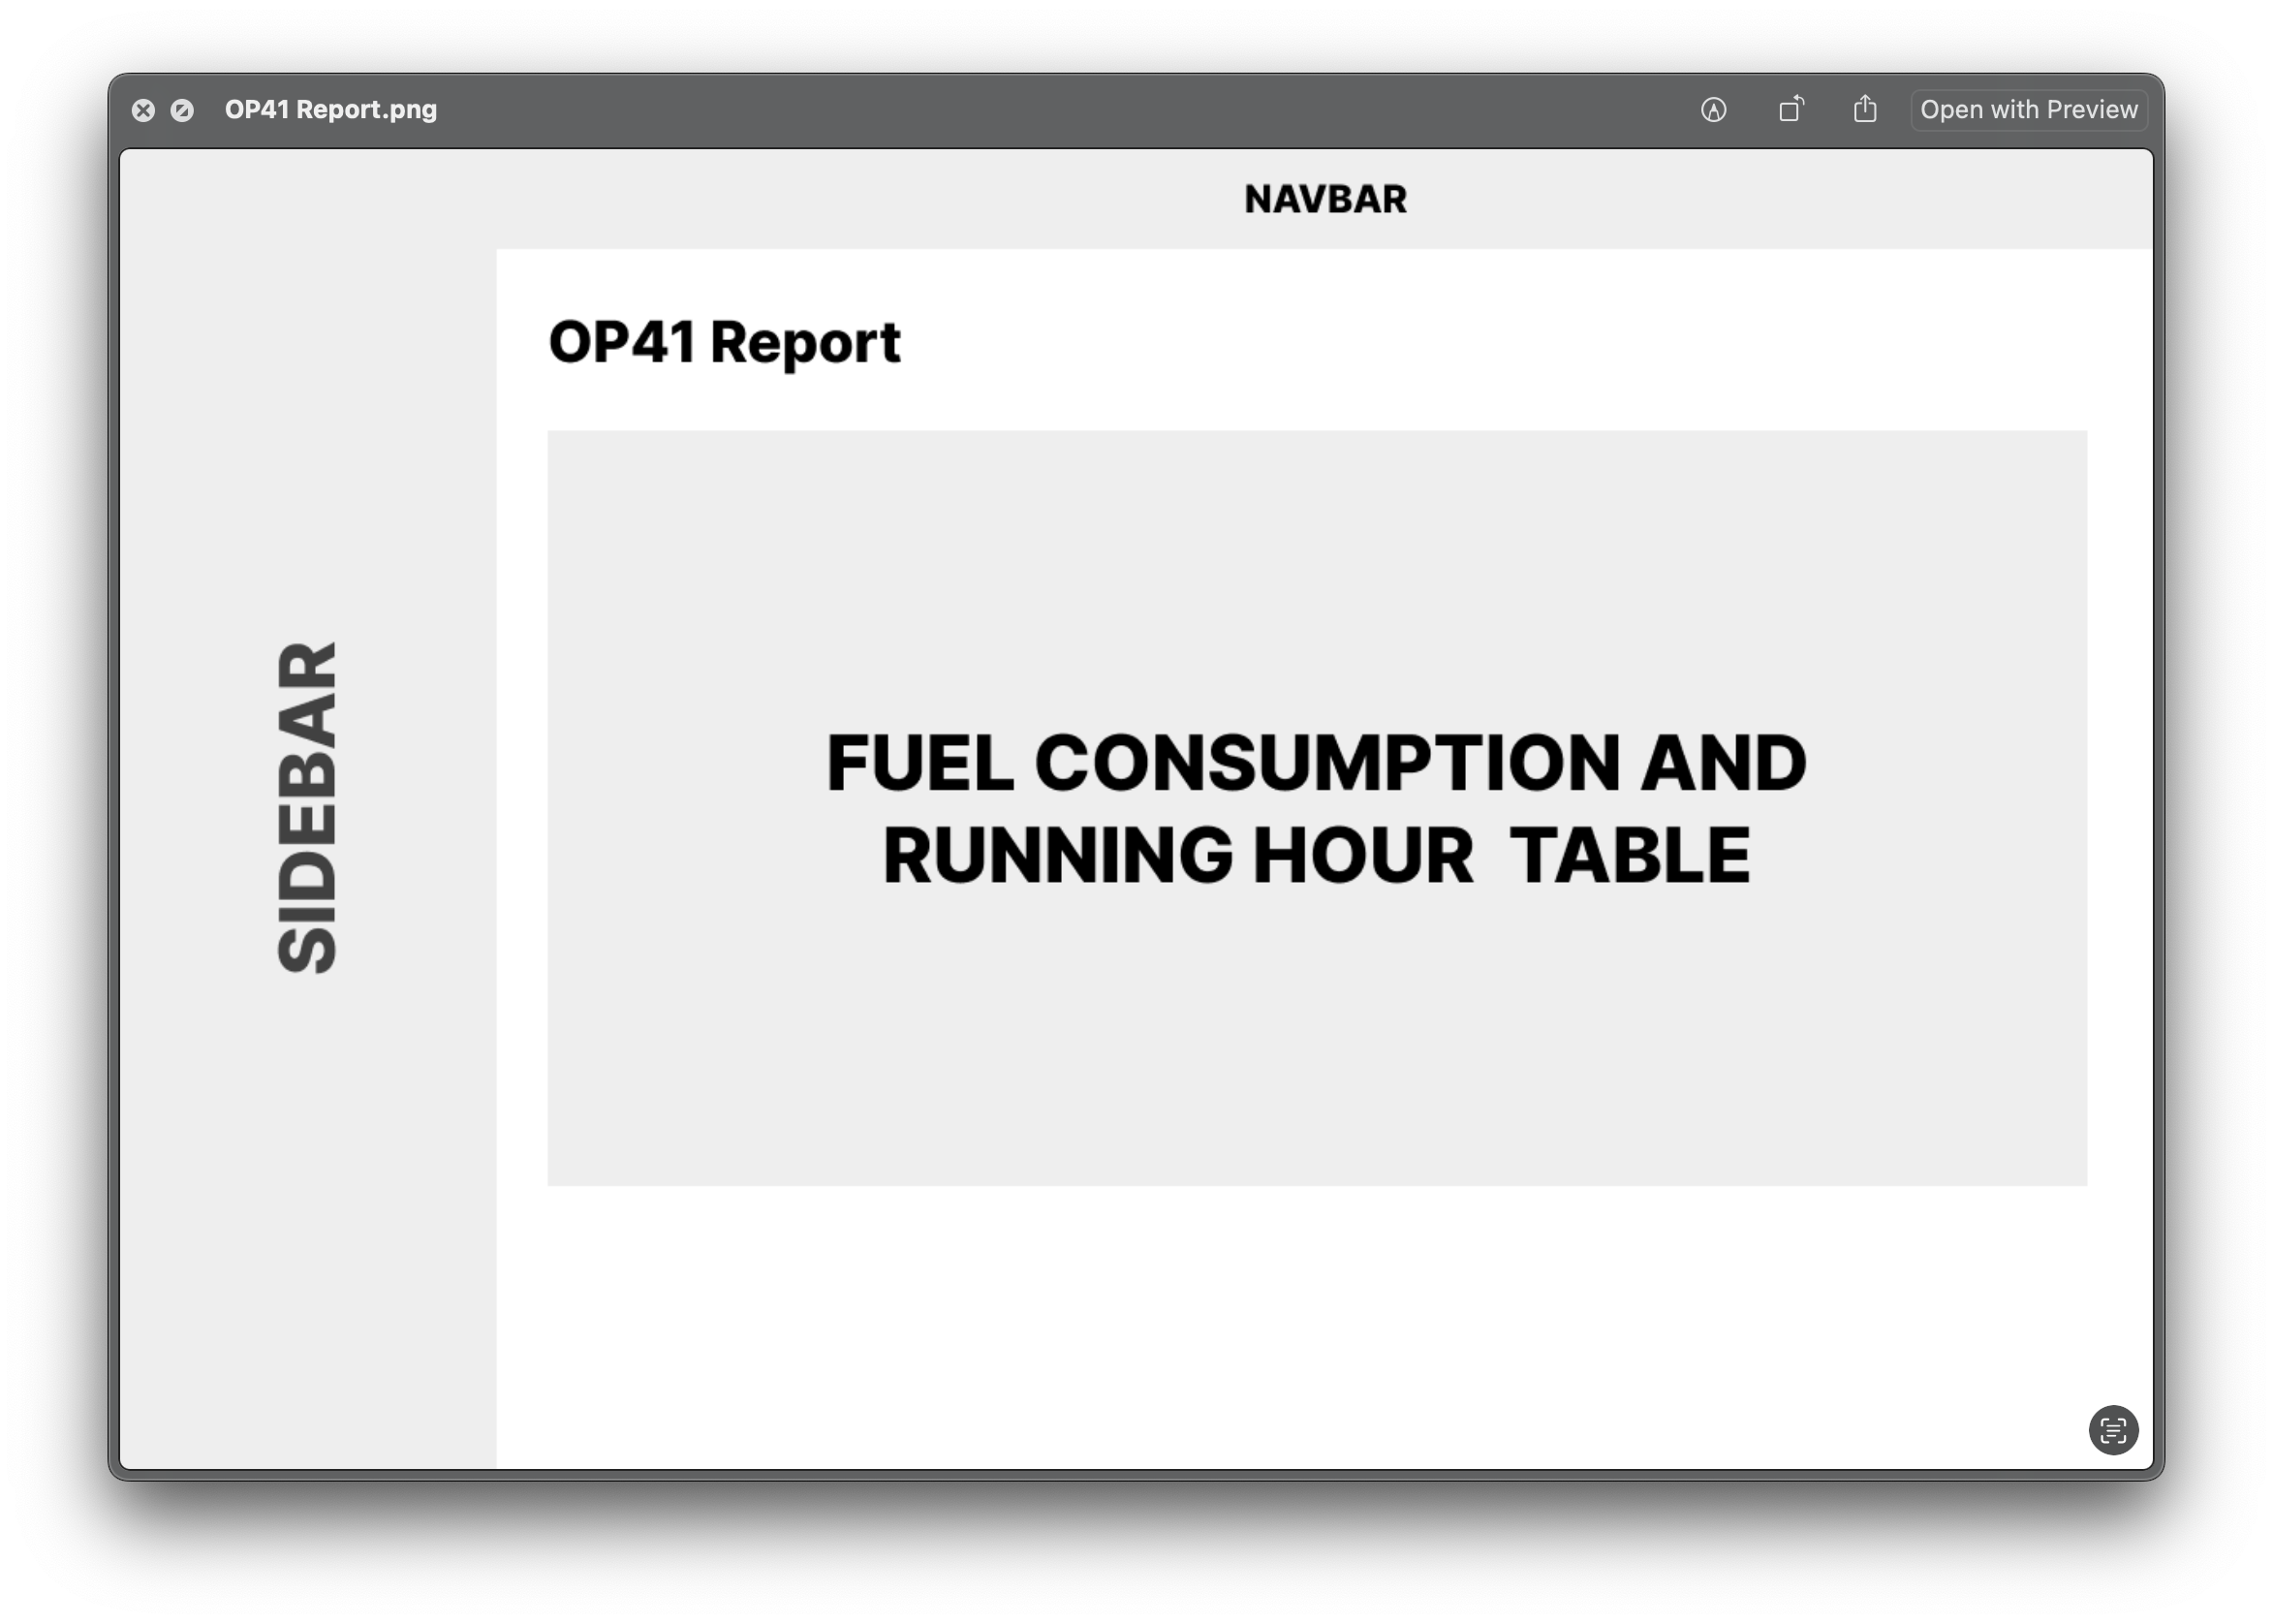
\includegraphics[width=1.05\linewidth, center]{images/hasil/iterations/1/lofi-op41.png}
%     \caption{Wireframe Halaman OP41 Report}
%     \label{fig:lofi-op41}
% \end{figure}

% \begin{figure}[!h]
%     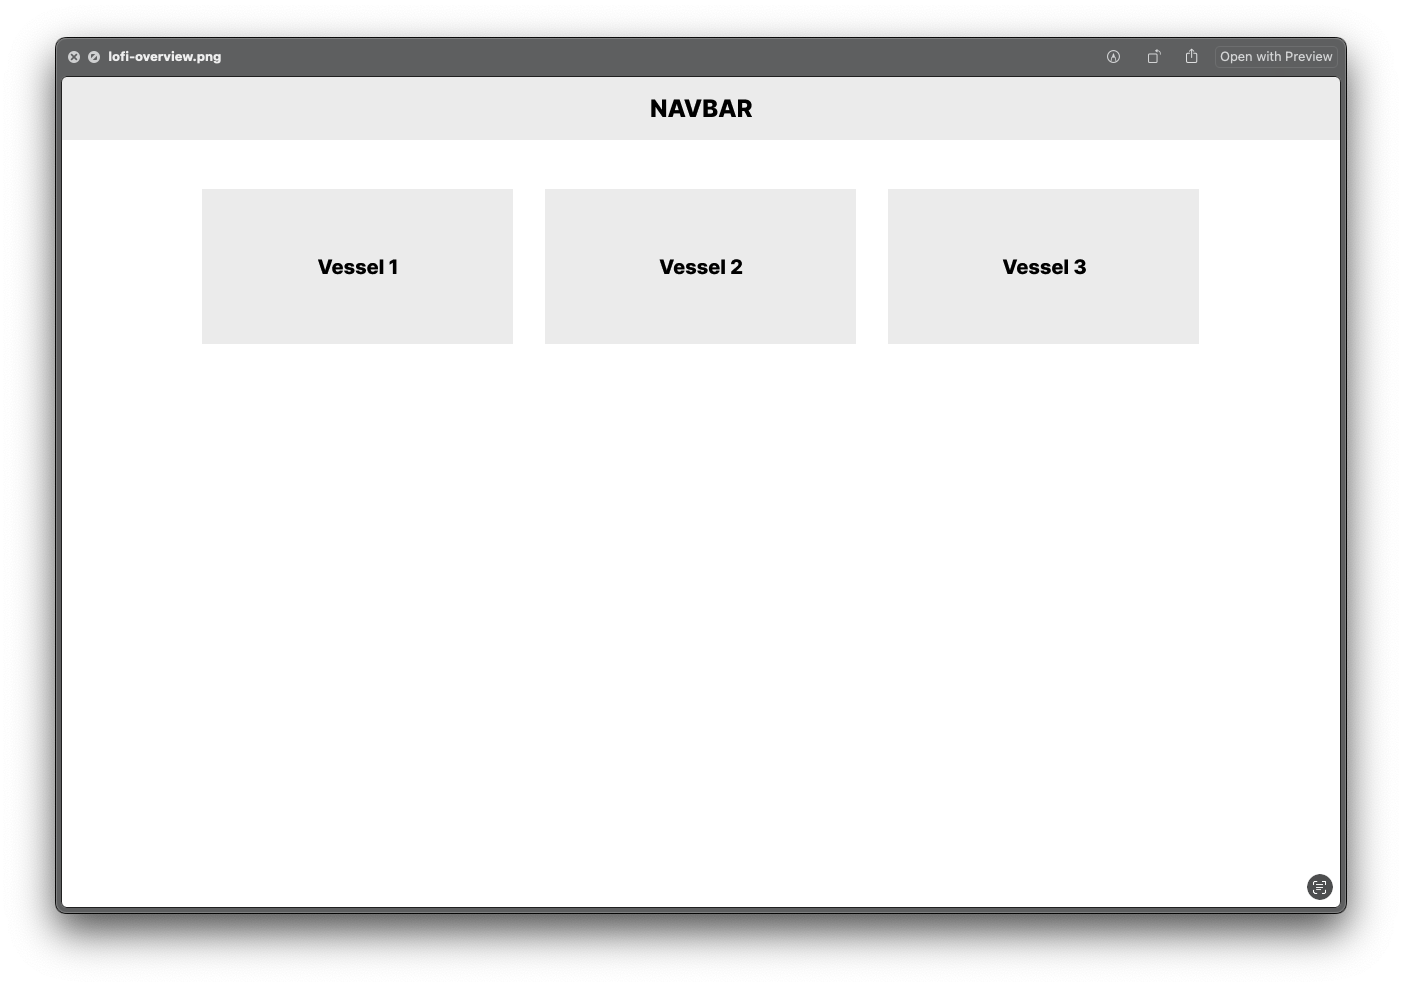
\includegraphics[width=1.05\linewidth, center]{images/hasil/iterations/5/lofi-overview.png}
%     \caption{Wireframe Halaman Overview}
%     \label{fig:lofi-overview}
% \end{figure}

% \newpage

% \subsubsection{Coding}

% Halaman OP41 memuat informasi running hour dan fuel consumption pada tiap kategori operasi berdasarkan Dokumen FCRV yang dapat menjadi acuan awak kapal untuk mengisi laporan. Jika data belum masuk semua maka ditampilkan alert agar awak kapal tidak mengisi laporan sebelum data pada hari tersebut telah tersinkron. Halaman OP41 dapat dilihat pada Gambar \ref{fig:fe-op41}.

% \begin{figure}[!h]
%     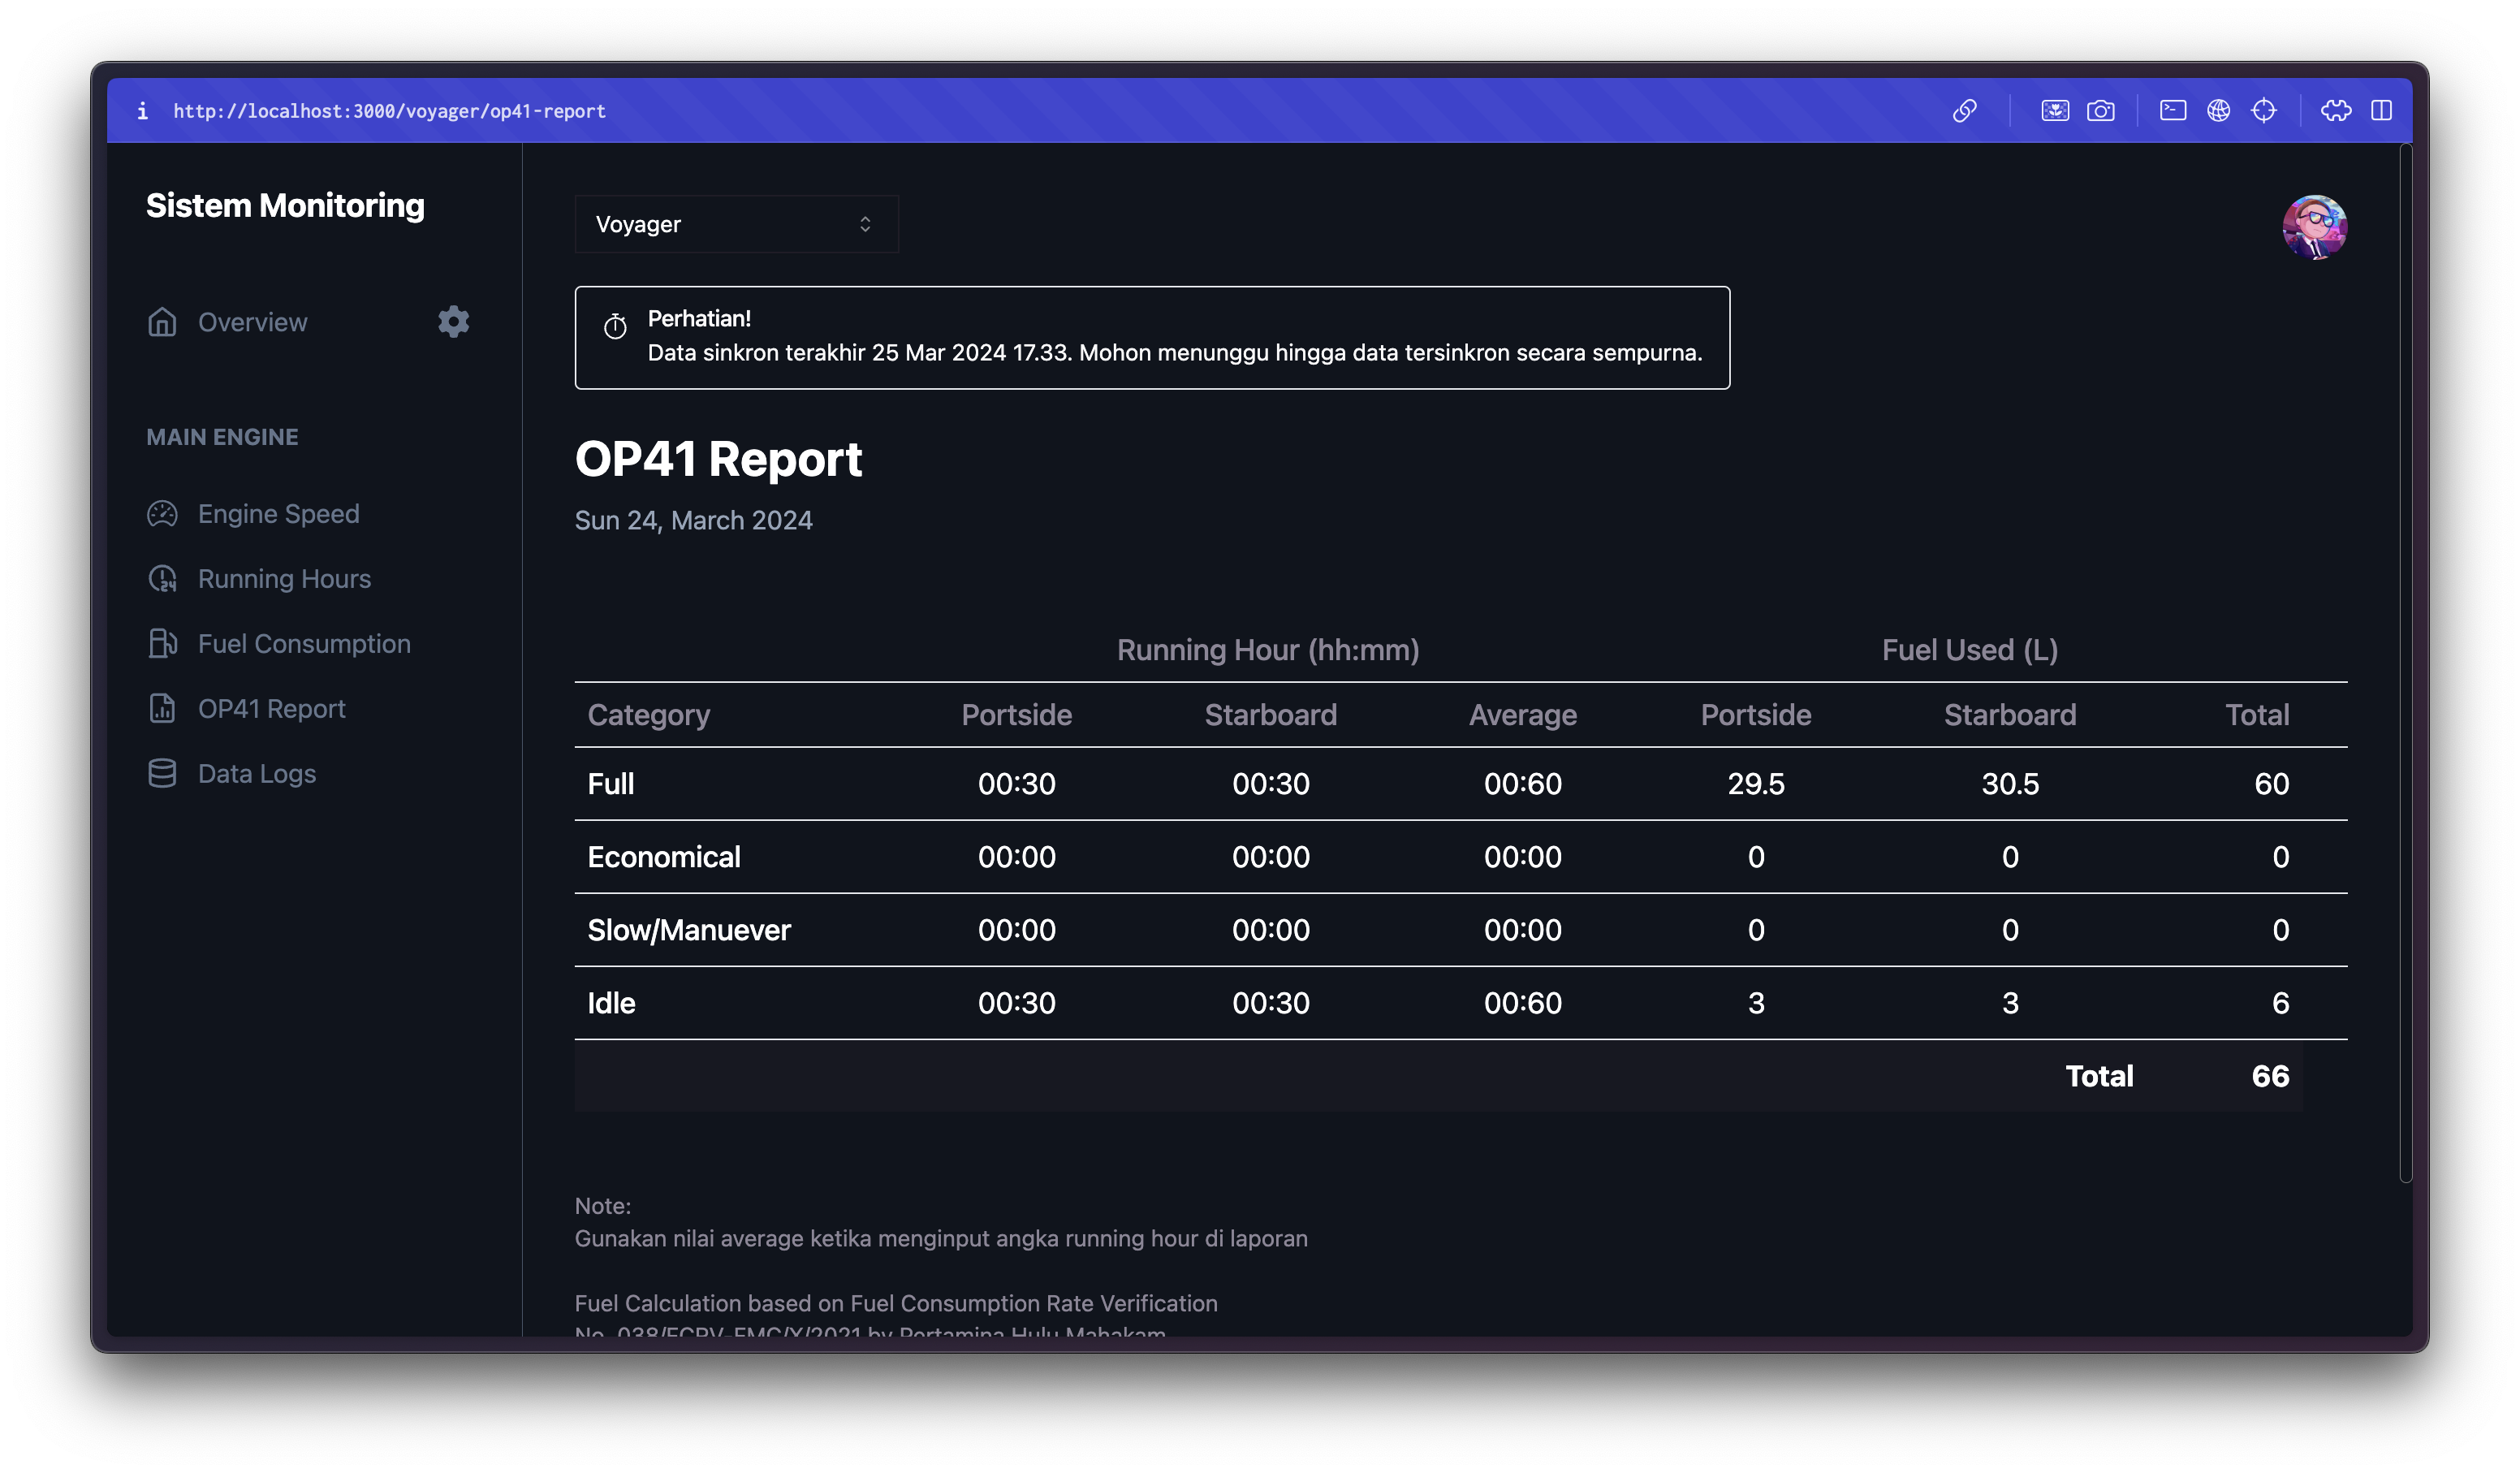
\includegraphics[width=1\linewidth, center]{images/hasil/iterations/5/fe-op41.png}
%     \caption{Frontend OP41 Report}
%     \label{fig:fe-op41}
% \end{figure}

% \newpage

% \subsubsection{Whitebox Testing}

% \begin{landscape}
%     \subsubsection{Blackbox Testing}

%     \begin{longtable}[!h]
    {
            p{0.2\textwidth}
            p{0.3\textwidth}
            p{0.3\textwidth}
            p{0.3\textwidth}
            p{0.3\textwidth}
            p{0.15\textwidth}
    }
    \caption{Blackbox Testing Ekspor Data Log Kecepatan Mesin}
    \label{tab:it4-blackbox-generate-es-report} \\

    \hline
        \bfseries \textit{Test Code} &
        \bfseries \textit{Test Case} &
        \bfseries \textit{Test Steps} &
        \bfseries \textit{Expected Result} &
        \bfseries \textit{Actual Result} &
        \bfseries \textit{Pass/Fail} \\ [0.5ex]
    \hline

    \endfirsthead

    \hline
        \bfseries \textit{Test Code} &
        \bfseries \textit{Test Case} &
        \bfseries \textit{Test Steps} &
        \bfseries \textit{Expected Result} &
        \bfseries \textit{Actual Result} &
        \bfseries \textit{Pass/Fail} \\ [0.5ex]
    \hline
    \endhead % all the lines above this will be repeated on every page
    \hline

    \csvreader[
        late after line=\\,
        before reading={\catcode`\#=12},after reading={\catcode`\#=6}
    ]{tables/hasil/iterations/5/blackbox/export-data.csv}
    {1=\code, 2=\case, 3=\step, 4=\expect, 5=\actual, 6=\status}
    {\code & \case & \step & \expect & \actual & \status} \\

    \bottomrule
\end{longtable}
%     \newpage
%     \begin{longtable}[!h]
    {
            p{0.2\textwidth}
            p{0.3\textwidth}
            p{0.3\textwidth}
            p{0.3\textwidth}
            p{0.3\textwidth}
            p{0.15\textwidth}
    }
    \caption{Blackbox Testing Halaman Autentikasi}
    \label{tab:it3-blackbox-auth-admin} \\

    \hline
        \bfseries \textit{Test Code} &
        \bfseries \textit{Test Case} &
        \bfseries \textit{Test Steps} &
        \bfseries \textit{Expected Result} &
        \bfseries \textit{Actual Result} &
        \bfseries \textit{Pass/Fail} \\ [0.5ex]
    \hline

    \endfirsthead

    \hline
        \bfseries \textit{Test Code} &
        \bfseries \textit{Test Case} &
        \bfseries \textit{Test Steps} &
        \bfseries \textit{Expected Result} &
        \bfseries \textit{Actual Result} &
        \bfseries \textit{Pass/Fail} \\ [0.5ex]
    \hline
    \endhead % all the lines above this will be repeated on every page
    \hline

    \csvreader[
        late after line=\\,
        before reading={\catcode`\#=12},after reading={\catcode`\#=6}
    ]{tables/hasil/iterations/3/blackbox/autentikasi.csv}
    {1=\code, 2=\case, 3=\step, 4=\expect, 5=\actual, 6=\status}
    {\code & \case & \step & \expect & \actual & \status} \\

    \bottomrule
\end{longtable}

% \end{landscape}